% Options for packages loaded elsewhere
\PassOptionsToPackage{unicode}{hyperref}
\PassOptionsToPackage{hyphens}{url}
%
\documentclass[
]{book}
\usepackage{amsmath,amssymb}
\usepackage{iftex}
\ifPDFTeX
  \usepackage[T1]{fontenc}
  \usepackage[utf8]{inputenc}
  \usepackage{textcomp} % provide euro and other symbols
\else % if luatex or xetex
  \usepackage{unicode-math} % this also loads fontspec
  \defaultfontfeatures{Scale=MatchLowercase}
  \defaultfontfeatures[\rmfamily]{Ligatures=TeX,Scale=1}
\fi
\usepackage{lmodern}
\ifPDFTeX\else
  % xetex/luatex font selection
\fi
% Use upquote if available, for straight quotes in verbatim environments
\IfFileExists{upquote.sty}{\usepackage{upquote}}{}
\IfFileExists{microtype.sty}{% use microtype if available
  \usepackage[]{microtype}
  \UseMicrotypeSet[protrusion]{basicmath} % disable protrusion for tt fonts
}{}
\makeatletter
\@ifundefined{KOMAClassName}{% if non-KOMA class
  \IfFileExists{parskip.sty}{%
    \usepackage{parskip}
  }{% else
    \setlength{\parindent}{0pt}
    \setlength{\parskip}{6pt plus 2pt minus 1pt}}
}{% if KOMA class
  \KOMAoptions{parskip=half}}
\makeatother
\usepackage{xcolor}
\usepackage{color}
\usepackage{fancyvrb}
\newcommand{\VerbBar}{|}
\newcommand{\VERB}{\Verb[commandchars=\\\{\}]}
\DefineVerbatimEnvironment{Highlighting}{Verbatim}{commandchars=\\\{\}}
% Add ',fontsize=\small' for more characters per line
\usepackage{framed}
\definecolor{shadecolor}{RGB}{248,248,248}
\newenvironment{Shaded}{\begin{snugshade}}{\end{snugshade}}
\newcommand{\AlertTok}[1]{\textcolor[rgb]{0.94,0.16,0.16}{#1}}
\newcommand{\AnnotationTok}[1]{\textcolor[rgb]{0.56,0.35,0.01}{\textbf{\textit{#1}}}}
\newcommand{\AttributeTok}[1]{\textcolor[rgb]{0.13,0.29,0.53}{#1}}
\newcommand{\BaseNTok}[1]{\textcolor[rgb]{0.00,0.00,0.81}{#1}}
\newcommand{\BuiltInTok}[1]{#1}
\newcommand{\CharTok}[1]{\textcolor[rgb]{0.31,0.60,0.02}{#1}}
\newcommand{\CommentTok}[1]{\textcolor[rgb]{0.56,0.35,0.01}{\textit{#1}}}
\newcommand{\CommentVarTok}[1]{\textcolor[rgb]{0.56,0.35,0.01}{\textbf{\textit{#1}}}}
\newcommand{\ConstantTok}[1]{\textcolor[rgb]{0.56,0.35,0.01}{#1}}
\newcommand{\ControlFlowTok}[1]{\textcolor[rgb]{0.13,0.29,0.53}{\textbf{#1}}}
\newcommand{\DataTypeTok}[1]{\textcolor[rgb]{0.13,0.29,0.53}{#1}}
\newcommand{\DecValTok}[1]{\textcolor[rgb]{0.00,0.00,0.81}{#1}}
\newcommand{\DocumentationTok}[1]{\textcolor[rgb]{0.56,0.35,0.01}{\textbf{\textit{#1}}}}
\newcommand{\ErrorTok}[1]{\textcolor[rgb]{0.64,0.00,0.00}{\textbf{#1}}}
\newcommand{\ExtensionTok}[1]{#1}
\newcommand{\FloatTok}[1]{\textcolor[rgb]{0.00,0.00,0.81}{#1}}
\newcommand{\FunctionTok}[1]{\textcolor[rgb]{0.13,0.29,0.53}{\textbf{#1}}}
\newcommand{\ImportTok}[1]{#1}
\newcommand{\InformationTok}[1]{\textcolor[rgb]{0.56,0.35,0.01}{\textbf{\textit{#1}}}}
\newcommand{\KeywordTok}[1]{\textcolor[rgb]{0.13,0.29,0.53}{\textbf{#1}}}
\newcommand{\NormalTok}[1]{#1}
\newcommand{\OperatorTok}[1]{\textcolor[rgb]{0.81,0.36,0.00}{\textbf{#1}}}
\newcommand{\OtherTok}[1]{\textcolor[rgb]{0.56,0.35,0.01}{#1}}
\newcommand{\PreprocessorTok}[1]{\textcolor[rgb]{0.56,0.35,0.01}{\textit{#1}}}
\newcommand{\RegionMarkerTok}[1]{#1}
\newcommand{\SpecialCharTok}[1]{\textcolor[rgb]{0.81,0.36,0.00}{\textbf{#1}}}
\newcommand{\SpecialStringTok}[1]{\textcolor[rgb]{0.31,0.60,0.02}{#1}}
\newcommand{\StringTok}[1]{\textcolor[rgb]{0.31,0.60,0.02}{#1}}
\newcommand{\VariableTok}[1]{\textcolor[rgb]{0.00,0.00,0.00}{#1}}
\newcommand{\VerbatimStringTok}[1]{\textcolor[rgb]{0.31,0.60,0.02}{#1}}
\newcommand{\WarningTok}[1]{\textcolor[rgb]{0.56,0.35,0.01}{\textbf{\textit{#1}}}}
\usepackage{longtable,booktabs,array}
\usepackage{calc} % for calculating minipage widths
% Correct order of tables after \paragraph or \subparagraph
\usepackage{etoolbox}
\makeatletter
\patchcmd\longtable{\par}{\if@noskipsec\mbox{}\fi\par}{}{}
\makeatother
% Allow footnotes in longtable head/foot
\IfFileExists{footnotehyper.sty}{\usepackage{footnotehyper}}{\usepackage{footnote}}
\makesavenoteenv{longtable}
\usepackage{graphicx}
\makeatletter
\def\maxwidth{\ifdim\Gin@nat@width>\linewidth\linewidth\else\Gin@nat@width\fi}
\def\maxheight{\ifdim\Gin@nat@height>\textheight\textheight\else\Gin@nat@height\fi}
\makeatother
% Scale images if necessary, so that they will not overflow the page
% margins by default, and it is still possible to overwrite the defaults
% using explicit options in \includegraphics[width, height, ...]{}
\setkeys{Gin}{width=\maxwidth,height=\maxheight,keepaspectratio}
% Set default figure placement to htbp
\makeatletter
\def\fps@figure{htbp}
\makeatother
\setlength{\emergencystretch}{3em} % prevent overfull lines
\providecommand{\tightlist}{%
  \setlength{\itemsep}{0pt}\setlength{\parskip}{0pt}}
\setcounter{secnumdepth}{5}
\usepackage{booktabs}
\usepackage{amsthm}
\makeatletter
\def\thm@space@setup{%
  \thm@preskip=8pt plus 2pt minus 4pt
  \thm@postskip=\thm@preskip
}
\makeatother
\usepackage{booktabs}
\usepackage{longtable}
\usepackage{array}
\usepackage{multirow}
\usepackage{wrapfig}
\usepackage{float}
\usepackage{colortbl}
\usepackage{pdflscape}
\usepackage{tabu}
\usepackage{threeparttable}
\usepackage{threeparttablex}
\usepackage[normalem]{ulem}
\usepackage{makecell}
\usepackage{xcolor}
\ifLuaTeX
  \usepackage{selnolig}  % disable illegal ligatures
\fi
\usepackage[]{natbib}
\bibliographystyle{apalike}
\IfFileExists{bookmark.sty}{\usepackage{bookmark}}{\usepackage{hyperref}}
\IfFileExists{xurl.sty}{\usepackage{xurl}}{} % add URL line breaks if available
\urlstyle{same}
\hypersetup{
  pdftitle={rechaRge: the HydroBudget model},
  pdfauthor={Emmanuel Dubois, Yannick Marcon},
  hidelinks,
  pdfcreator={LaTeX via pandoc}}

\title{rechaRge: the HydroBudget model}
\author{Emmanuel Dubois, Yannick Marcon}
\date{2024-04-03}

\begin{document}
\maketitle

{
\setcounter{tocdepth}{1}
\tableofcontents
}
\hypertarget{welcome}{%
\chapter*{Welcome}\label{welcome}}
\addcontentsline{toc}{chapter}{Welcome}

This book provides users with some common workflows for performing groundwater recharge modeling. This book will teach you how to use the \href{https://github.com/gwrecharge/rechaRge}{rechaRge} R package \citep{R-rechaRge}. This material serves as an online companion for the manuscript ``Simulation of long-term spatiotemporal variations in regional-scale groundwater recharge: contributions of a water budget approach in cold and humid climates'' \citep{hess-25-6567-2021}.

\textbf{HydroBudget} (HB) is a spatially distributed groundwater recharge (GWR) model that computes a superficial water budget on grid cells of regional-scale watersheds with outputs aggregated into monthly time steps and with limited computational time. The model is open-source and was coded in R. This \texttt{rechaRge} R package is the result of the effort to make this code reusable and extensible.

This book is organized into three parts. In the \emph{Introduction}, we provide practical information about the \texttt{rechaRge} R package.

The \emph{Simulation} part focuses on the \textbf{HydroBudget} model that comes with the R package, and how make use the \texttt{rechaRge}functions to run simulations, then save and visualize the results.

The \emph{Calibration and Sensitivity} part explores the usage of the \texttt{sensitivity} and of the \texttt{caRamel} R packages to find and evaluate the ``best'' sets of model parameters.

Finally, the \emph{Extensibility} highlights how the generic functions of the \texttt{rechaRge} R package can applied to a different groundwater recharge model.

\hypertarget{intro}{%
\chapter{Introduction}\label{intro}}

\hypertarget{installation}{%
\section{Installation}\label{installation}}

The package will be submitted to the CRAN repository. In the meantime, the package installation options are:

\begin{itemize}
\tightlist
\item
  Using \texttt{remotes}
\end{itemize}

\begin{Shaded}
\begin{Highlighting}[]
\NormalTok{remotes}\SpecialCharTok{::}\FunctionTok{install\_github}\NormalTok{(}\StringTok{"gwrecharge/rechaRge"}\NormalTok{, }\AttributeTok{ref =} \StringTok{"main"}\NormalTok{)}
\end{Highlighting}
\end{Shaded}

\begin{itemize}
\tightlist
\item
  Using \texttt{pak}
\end{itemize}

\begin{Shaded}
\begin{Highlighting}[]
\NormalTok{pak}\SpecialCharTok{::}\FunctionTok{pkg\_install}\NormalTok{(}\StringTok{"gwrecharge/rechaRge@main"}\NormalTok{)}
\end{Highlighting}
\end{Shaded}

\hypertarget{usage}{%
\section{Usage}\label{usage}}

Some ready to use data files are made available for documentation and testing purposes. This book is based on these examples, see the section \ref{simulation}.

\hypertarget{simulation}{%
\chapter{Simulation}\label{simulation}}

\hypertarget{hydrobudget-model}{%
\section{HydroBudget Model}\label{hydrobudget-model}}

\textbf{HydroBudget} was developed as an accessible and computationally affordable model to simulate GWR over large areas (thousands of km2) and for long time periods (decades), in cold and humid climates. The model uses commonly available meteorological data (daily precipitation and temperature, spatialized if possible) and spatially distributed data (pedology, land cover, and slopes). It is calibrated with river flows and baseflows estimated with recursive filters. The model needs reasonable computational capacity to reach relatively short computational times. It is based on simplified representations of hydrological processes and is driven by eight parameters that need to be calibrated.

\textbf{HydroBudget} uses a degree-day snow model for snow accumulation and snowmelt, and a conceptual lumped reservoir to compute the soil water budget on a daily time step. For each grid cell and each time step, the calculation distributes precipitation as runoff (R), evapotranspiration (ET), and infiltration that can reach the saturated zone if geological conditions below the soil allow deep percolation. HB thus produces estimates of potential GWR. The daily results are compiled at a monthly time step.

\hypertarget{input-data-and-parameters}{%
\section{Input data and parameters}\label{input-data-and-parameters}}

Start with loading the \texttt{rechaRge} library.

\begin{Shaded}
\begin{Highlighting}[]
\FunctionTok{library}\NormalTok{(rechaRge)}
\end{Highlighting}
\end{Shaded}

Then load the input data for the simulation. In that case, the example datasets are available for download. The data input handler is based on \texttt{data.table::fread} function, then you can provide an URL like in the example or a local file path.

\begin{Shaded}
\begin{Highlighting}[]
\NormalTok{base\_url }\OtherTok{\textless{}{-}} \StringTok{"https://github.com/gwrecharge/rechaRge{-}book/raw/main/examples/input/"}
\NormalTok{input\_rcn }\OtherTok{\textless{}{-}} \FunctionTok{paste0}\NormalTok{(base\_url, }\StringTok{"rcn.csv.gz"}\NormalTok{) }\CommentTok{\# RCN values per RCN cell ID}
\NormalTok{input\_climate }\OtherTok{\textless{}{-}} \FunctionTok{paste0}\NormalTok{(base\_url, }\StringTok{"climate.csv.gz"}\NormalTok{) }\CommentTok{\# precipitation total in mm/d per climate cell ID}
\NormalTok{input\_rcn\_climate }\OtherTok{\textless{}{-}} \FunctionTok{paste0}\NormalTok{(base\_url, }\StringTok{"rcn\_climate.csv.gz"}\NormalTok{) }\CommentTok{\# relation between climate and RCN cell IDs}
\end{Highlighting}
\end{Shaded}

Set the \textbf{HydroBudget} model with the parameters values (if you do not know which parameters to set, see the Calibration section):

\begin{Shaded}
\begin{Highlighting}[]
\NormalTok{HB }\OtherTok{\textless{}{-}}\NormalTok{ rechaRge}\SpecialCharTok{::}\FunctionTok{new\_hydrobudget}\NormalTok{(}
  \AttributeTok{T\_m =} \FloatTok{2.1}\NormalTok{, }\CommentTok{\# melting temperature (°C)}
  \AttributeTok{C\_m =} \FloatTok{6.2}\NormalTok{, }\CommentTok{\# melting coefficient (mm/°C/d)}
  \AttributeTok{TT\_F =} \SpecialCharTok{{-}}\FloatTok{17.6}\NormalTok{, }\CommentTok{\# Threshold temperature for soil frost (°C)}
  \AttributeTok{F\_T =} \FloatTok{16.4}\NormalTok{, }\CommentTok{\# Freezing time (d)}
  \AttributeTok{t\_API =} \FloatTok{3.9}\NormalTok{, }\CommentTok{\# Antecedent precipitation index time (d)}
  \AttributeTok{f\_runoff =} \FloatTok{0.63}\NormalTok{, }\CommentTok{\# Runoff factor ({-})}
  \AttributeTok{sw\_m =} \DecValTok{431}\NormalTok{, }\CommentTok{\# Maximum soil water content (mm)}
  \AttributeTok{f\_inf =} \FloatTok{0.07} \CommentTok{\# infiltration factor ({-})}
\NormalTok{)}
\end{Highlighting}
\end{Shaded}

As the \textbf{HydroBudget} model expects some data structure (expected data, with predefined column names), set the column names mappings matching the input datasets:

\begin{Shaded}
\begin{Highlighting}[]
\NormalTok{HB}\SpecialCharTok{$}\NormalTok{rcn\_columns }\OtherTok{\textless{}{-}} \FunctionTok{list}\NormalTok{(}
  \AttributeTok{rcn\_id =} \StringTok{"cell\_ID"}\NormalTok{,}
  \AttributeTok{RCNII =} \StringTok{"RCNII"}\NormalTok{,}
  \AttributeTok{lon =} \StringTok{"X\_L93"}\NormalTok{,}
  \AttributeTok{lat =} \StringTok{"Y\_L93"}
\NormalTok{)}
\NormalTok{HB}\SpecialCharTok{$}\NormalTok{climate\_columns}\SpecialCharTok{$}\NormalTok{climate\_id }\OtherTok{\textless{}{-}} \StringTok{"climate\_cell"}
\NormalTok{HB}\SpecialCharTok{$}\NormalTok{rcn\_climate\_columns }\OtherTok{\textless{}{-}} \FunctionTok{list}\NormalTok{(}
  \AttributeTok{climate\_id =} \StringTok{"climate\_cell"}\NormalTok{,}
  \AttributeTok{rcn\_id =} \StringTok{"cell\_ID"}
\NormalTok{)}
\end{Highlighting}
\end{Shaded}

Then define the simulation period (if not, the period will be discovered from the input data):

\begin{Shaded}
\begin{Highlighting}[]
\NormalTok{simul\_period }\OtherTok{\textless{}{-}} \FunctionTok{c}\NormalTok{(}\DecValTok{2010}\NormalTok{, }\DecValTok{2017}\NormalTok{)}
\end{Highlighting}
\end{Shaded}

\hypertarget{simulation-1}{%
\section{Simulation}\label{simulation-1}}

Once the \textbf{HydroBudget} object is ready, compute the water budget using the model implementation:

\begin{Shaded}
\begin{Highlighting}[]
\NormalTok{water\_budget }\OtherTok{\textless{}{-}}\NormalTok{ rechaRge}\SpecialCharTok{::}\FunctionTok{compute\_recharge}\NormalTok{(}
\NormalTok{  HB,}
  \AttributeTok{rcn =}\NormalTok{ input\_rcn,}
  \AttributeTok{climate =}\NormalTok{ input\_climate,}
  \AttributeTok{rcn\_climate =}\NormalTok{ input\_rcn\_climate,}
  \AttributeTok{period =}\NormalTok{ simul\_period}
\NormalTok{)}
\end{Highlighting}
\end{Shaded}

The water budget data set is per year-month in each RCN cell:

\begin{itemize}
\tightlist
\item
  \texttt{vi}, the vertical inflow
\item
  \texttt{t\_mean}, the mean temperature
\item
  \texttt{runoff}, the runoff
\item
  \texttt{pet}, the potential evapotranspiration
\item
  \texttt{aet}, the actual evapotranspiration
\item
  \texttt{gwr}, the groundwater recharge
\item
  \texttt{runoff\_2}, the excess runoff
\end{itemize}

The head of this data set is:

\begin{tabular}{r|r|r|r|r|r|r|r|r|r|r}
\hline
year & month & vi & t\_mean & runoff & pet & aet & gwr & runoff\_2 & delta\_reservoir & rcn\_id\\
\hline
2010 & 1 & 28.2 & -7.3 & 21.5 & 1.6 & 1.6 & 10.2 & 0 & -5.1 & 62097\\
\hline
2010 & 2 & 27.9 & -5.7 & 7.9 & 4.6 & 4.6 & 8.8 & 0 & 6.6 & 62097\\
\hline
2010 & 3 & 83.0 & 1.0 & 30.8 & 19.5 & 19.5 & 16.1 & 0 & 16.6 & 62097\\
\hline
2010 & 4 & 68.2 & 7.7 & 24.9 & 51.5 & 51.5 & 15.1 & 0 & -23.3 & 62097\\
\hline
2010 & 5 & 46.9 & 13.8 & 3.8 & 94.7 & 73.8 & 4.4 & 0 & -35.2 & 62097\\
\hline
2010 & 6 & 107.9 & 17.0 & 33.3 & 114.7 & 81.1 & 0.2 & 0 & -6.7 & 62097\\
\hline
\end{tabular}

\hypertarget{results}{%
\section{Results}\label{results}}

The simulation results can be reworked, summarized and visualized.

\hypertarget{save-results-in-files}{%
\subsection{Save results in files}\label{save-results-in-files}}

Start with defining the output folder:

\begin{Shaded}
\begin{Highlighting}[]
\NormalTok{sim\_dir }\OtherTok{\textless{}{-}} \FunctionTok{file.path}\NormalTok{(}\FunctionTok{tempdir}\NormalTok{(), }\FunctionTok{paste0}\NormalTok{(}\StringTok{"simulation\_HydroBudget\_"}\NormalTok{, }\FunctionTok{format}\NormalTok{(}\FunctionTok{Sys.time}\NormalTok{(), }\StringTok{"\%Y\%m\%dT\%H\_\%M"}\NormalTok{)))}
\end{Highlighting}
\end{Shaded}

Then write the resulting water budget in different formats in this output folder:

\begin{itemize}
\tightlist
\item
  CSV
\end{itemize}

\begin{Shaded}
\begin{Highlighting}[]
\CommentTok{\# CSV}
\NormalTok{rechaRge}\SpecialCharTok{::}\FunctionTok{write\_recharge\_results}\NormalTok{(HB, water\_budget, }\AttributeTok{output\_dir =}\NormalTok{ sim\_dir)}
\end{Highlighting}
\end{Shaded}

\begin{itemize}
\tightlist
\item
  NetCDF
\end{itemize}

\begin{Shaded}
\begin{Highlighting}[]
\CommentTok{\# NetCDF}
\NormalTok{rechaRge}\SpecialCharTok{::}\FunctionTok{write\_recharge\_results}\NormalTok{(HB, water\_budget, }\AttributeTok{output\_dir =}\NormalTok{ sim\_dir, }\AttributeTok{format =} \StringTok{"nc"}\NormalTok{, }\AttributeTok{input\_rcn =}\NormalTok{ input\_rcn, }\AttributeTok{names =} \FunctionTok{list}\NormalTok{(}
  \StringTok{"lon"} \OtherTok{=} \FunctionTok{list}\NormalTok{(}
    \AttributeTok{longname =} \StringTok{"Qc lambert NAD83 epsg32198 Est"}\NormalTok{,}
    \AttributeTok{unit =} \StringTok{"m"}
\NormalTok{  ),}
  \StringTok{"lat"} \OtherTok{=} \FunctionTok{list}\NormalTok{(}
    \AttributeTok{longname =} \StringTok{"Qc lambert NAD83 epsg32198 North"}\NormalTok{,}
    \AttributeTok{unit =} \StringTok{"m"}
\NormalTok{  )}
\NormalTok{))}
\end{Highlighting}
\end{Shaded}

\begin{itemize}
\tightlist
\item
  Rasters
\end{itemize}

\begin{Shaded}
\begin{Highlighting}[]
\CommentTok{\# Rasters}
\NormalTok{rechaRge}\SpecialCharTok{::}\FunctionTok{write\_recharge\_rasters}\NormalTok{(}
\NormalTok{  HB,}
  \AttributeTok{water\_budget =}\NormalTok{ water\_budget,}
  \AttributeTok{input\_rcn =}\NormalTok{ input\_rcn,}
  \AttributeTok{crs =} \StringTok{"+proj=lcc +lat\_1=60 +lat\_2=46 +lat\_0=44 +lon\_0={-}68.5 +x\_0=0 +y\_0=0 +ellps=GRS80 +datum=NAD83 +units=m +no\_defs"}\NormalTok{,}
  \AttributeTok{output\_dir =}\NormalTok{ sim\_dir}
\NormalTok{)}
\end{Highlighting}
\end{Shaded}

The output folder content should look like this:

\begin{Shaded}
\begin{Highlighting}[]
\CommentTok{\# List simulation output files}
\FunctionTok{list.files}\NormalTok{(sim\_dir)}
\end{Highlighting}
\end{Shaded}

\begin{verbatim}
[1] "bilan_spat_month.csv"         "bilan_unspat_month.csv"      
[3] "interannual_aet_NAD83.tif"    "interannual_gwr_NAD83.tif"   
[5] "interannual_runoff_NAD83.tif" "water_budget.nc"             
\end{verbatim}

\hypertarget{data-visualization}{%
\subsection{Data visualization}\label{data-visualization}}

Visualize the saved NetCDF file:

\begin{Shaded}
\begin{Highlighting}[]
\FunctionTok{library}\NormalTok{(ncdf4)}
\FunctionTok{library}\NormalTok{(lattice)}
\FunctionTok{library}\NormalTok{(viridisLite)}

\CommentTok{\# Extract GWR data}
\NormalTok{nc }\OtherTok{\textless{}{-}} \FunctionTok{nc\_open}\NormalTok{(}\FunctionTok{file.path}\NormalTok{(sim\_dir, }\StringTok{"water\_budget.nc"}\NormalTok{))}
\NormalTok{gwr }\OtherTok{\textless{}{-}} \FunctionTok{ncvar\_get}\NormalTok{(nc, }\StringTok{"gwr"}\NormalTok{)}
\NormalTok{gwratt }\OtherTok{\textless{}{-}} \FunctionTok{ncatt\_get}\NormalTok{(nc, }\StringTok{"gwr"}\NormalTok{)}
\NormalTok{lon }\OtherTok{\textless{}{-}} \FunctionTok{ncvar\_get}\NormalTok{(nc, }\StringTok{"lon"}\NormalTok{)}
\NormalTok{lonatt }\OtherTok{\textless{}{-}} \FunctionTok{ncatt\_get}\NormalTok{(nc, }\StringTok{"lon"}\NormalTok{)}
\NormalTok{lat }\OtherTok{\textless{}{-}} \FunctionTok{ncvar\_get}\NormalTok{(nc, }\StringTok{"lat"}\NormalTok{)}
\NormalTok{latatt }\OtherTok{\textless{}{-}} \FunctionTok{ncatt\_get}\NormalTok{(nc, }\StringTok{"lat"}\NormalTok{)}
\NormalTok{time }\OtherTok{\textless{}{-}} \FunctionTok{ncvar\_get}\NormalTok{(nc, }\StringTok{"time"}\NormalTok{)}
\FunctionTok{nc\_close}\NormalTok{(nc)}

\CommentTok{\# Render the 18th month}
\NormalTok{month }\OtherTok{\textless{}{-}} \DecValTok{18}
\NormalTok{gwr1 }\OtherTok{\textless{}{-}}\NormalTok{ gwr[,,month]}
\NormalTok{grid }\OtherTok{\textless{}{-}} \FunctionTok{expand.grid}\NormalTok{(}\AttributeTok{lon=}\NormalTok{lon, }\AttributeTok{lat=}\NormalTok{lat)}
\NormalTok{title }\OtherTok{\textless{}{-}} \FunctionTok{paste0}\NormalTok{(gwratt}\SpecialCharTok{$}\NormalTok{long\_name, }\StringTok{" ("}\NormalTok{, gwratt}\SpecialCharTok{$}\NormalTok{units, }\StringTok{") "}\NormalTok{, }\StringTok{" \#"}\NormalTok{, month)}
\NormalTok{xlab }\OtherTok{\textless{}{-}} \FunctionTok{paste0}\NormalTok{(latatt}\SpecialCharTok{$}\NormalTok{long\_name, }\StringTok{" ("}\NormalTok{, latatt}\SpecialCharTok{$}\NormalTok{units, }\StringTok{")"}\NormalTok{)}
\NormalTok{ylab }\OtherTok{\textless{}{-}} \FunctionTok{paste0}\NormalTok{(lonatt}\SpecialCharTok{$}\NormalTok{long\_name, }\StringTok{" ("}\NormalTok{, lonatt}\SpecialCharTok{$}\NormalTok{units, }\StringTok{")"}\NormalTok{)}
\FunctionTok{levelplot}\NormalTok{(gwr1 }\SpecialCharTok{\textasciitilde{}}\NormalTok{ lon }\SpecialCharTok{*}\NormalTok{ lat, }\AttributeTok{data=}\NormalTok{grid, }\AttributeTok{pretty=}\NormalTok{T, }\AttributeTok{col.regions=}\FunctionTok{inferno}\NormalTok{(}\DecValTok{100}\NormalTok{),}
          \AttributeTok{main=}\NormalTok{title, }\AttributeTok{xlab=}\NormalTok{xlab, }\AttributeTok{ylab=}\NormalTok{ylab)}
\end{Highlighting}
\end{Shaded}

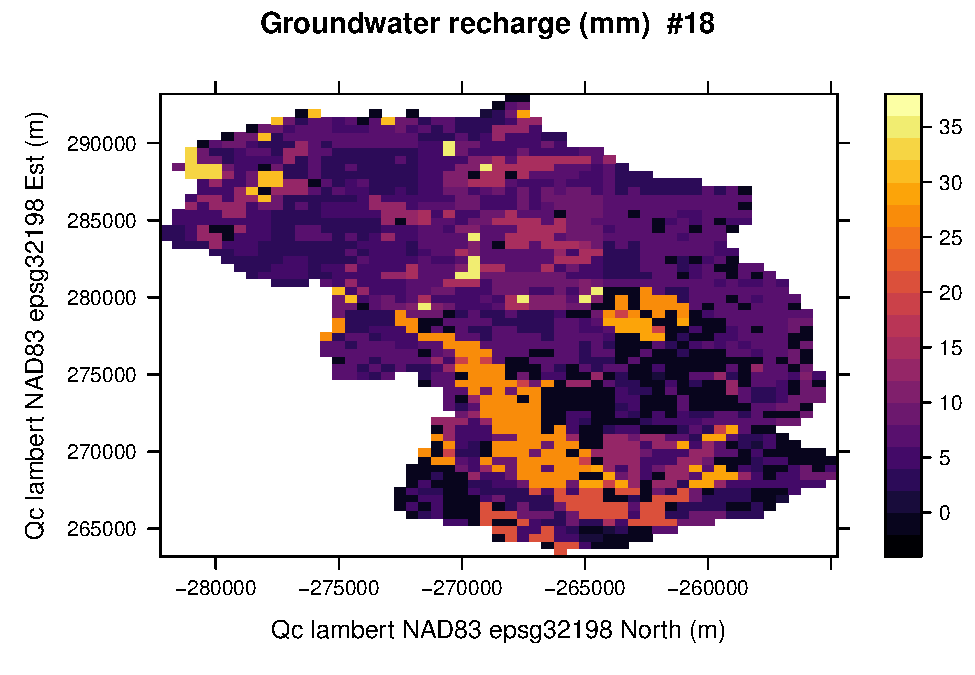
\includegraphics{fig/sim-viz-nc-1.pdf}

Visualize the saved raster files:

\begin{Shaded}
\begin{Highlighting}[]
\FunctionTok{library}\NormalTok{(tidyterra)}
\FunctionTok{library}\NormalTok{(terra)}
\FunctionTok{library}\NormalTok{(ggplot2)}
\FunctionTok{library}\NormalTok{(cowplot)}
\NormalTok{subtitle }\OtherTok{\textless{}{-}} \FunctionTok{ifelse}\NormalTok{(simul\_period[}\DecValTok{1}\NormalTok{] }\SpecialCharTok{==}\NormalTok{ simul\_period[}\DecValTok{2}\NormalTok{],}
  \FunctionTok{paste0}\NormalTok{(}\StringTok{"In "}\NormalTok{, simul\_period[}\DecValTok{1}\NormalTok{]),}
  \FunctionTok{paste0}\NormalTok{(}\StringTok{"From "}\NormalTok{, simul\_period[}\DecValTok{1}\NormalTok{], }\StringTok{" to "}\NormalTok{, simul\_period[}\DecValTok{2}\NormalTok{])}
\NormalTok{)}
\NormalTok{runoff }\OtherTok{\textless{}{-}}\NormalTok{ terra}\SpecialCharTok{::}\FunctionTok{rast}\NormalTok{(}\FunctionTok{file.path}\NormalTok{(sim\_dir, }\StringTok{"interannual\_runoff\_NAD83.tif"}\NormalTok{))}
\NormalTok{runoffplot }\OtherTok{\textless{}{-}} \FunctionTok{ggplot}\NormalTok{() }\SpecialCharTok{+}
  \FunctionTok{geom\_spatraster}\NormalTok{(}\AttributeTok{data =}\NormalTok{ runoff) }\SpecialCharTok{+}
  \FunctionTok{scale\_fill\_viridis\_c}\NormalTok{(}\AttributeTok{option =} \StringTok{"inferno"}\NormalTok{) }\SpecialCharTok{+}
  \FunctionTok{labs}\NormalTok{(}
    \AttributeTok{fill =} \StringTok{""}\NormalTok{,}
    \AttributeTok{title =} \StringTok{"Runoff"}\NormalTok{,}
    \AttributeTok{subtitle =}\NormalTok{ subtitle}
\NormalTok{  )}
\NormalTok{aet }\OtherTok{\textless{}{-}}\NormalTok{ terra}\SpecialCharTok{::}\FunctionTok{rast}\NormalTok{(}\FunctionTok{file.path}\NormalTok{(sim\_dir, }\StringTok{"interannual\_aet\_NAD83.tif"}\NormalTok{))}
\NormalTok{aetplot }\OtherTok{\textless{}{-}} \FunctionTok{ggplot}\NormalTok{() }\SpecialCharTok{+}
  \FunctionTok{geom\_spatraster}\NormalTok{(}\AttributeTok{data =}\NormalTok{ aet) }\SpecialCharTok{+}
  \FunctionTok{scale\_fill\_viridis\_c}\NormalTok{(}\AttributeTok{option =} \StringTok{"inferno"}\NormalTok{) }\SpecialCharTok{+}
  \FunctionTok{labs}\NormalTok{(}
    \AttributeTok{fill =} \StringTok{""}\NormalTok{,}
    \AttributeTok{title =} \StringTok{"Actual Evapotranspiration"}\NormalTok{,}
    \AttributeTok{subtitle =}\NormalTok{ subtitle}
\NormalTok{  )}
\NormalTok{gwr }\OtherTok{\textless{}{-}}\NormalTok{ terra}\SpecialCharTok{::}\FunctionTok{rast}\NormalTok{(}\FunctionTok{file.path}\NormalTok{(sim\_dir, }\StringTok{"interannual\_gwr\_NAD83.tif"}\NormalTok{))}
\NormalTok{gwrplot }\OtherTok{\textless{}{-}} \FunctionTok{ggplot}\NormalTok{() }\SpecialCharTok{+}
  \FunctionTok{geom\_spatraster}\NormalTok{(}\AttributeTok{data =}\NormalTok{ gwr) }\SpecialCharTok{+}
  \FunctionTok{scale\_fill\_viridis\_c}\NormalTok{(}\AttributeTok{option =} \StringTok{"inferno"}\NormalTok{) }\SpecialCharTok{+}
  \FunctionTok{labs}\NormalTok{(}
    \AttributeTok{fill =} \StringTok{""}\NormalTok{,}
    \AttributeTok{title =} \StringTok{"Groundwater Recharge"}\NormalTok{,}
    \AttributeTok{subtitle =}\NormalTok{ subtitle}
\NormalTok{  )}
\NormalTok{cowplot}\SpecialCharTok{::}\FunctionTok{plot\_grid}\NormalTok{(runoffplot, aetplot, gwrplot)}
\end{Highlighting}
\end{Shaded}

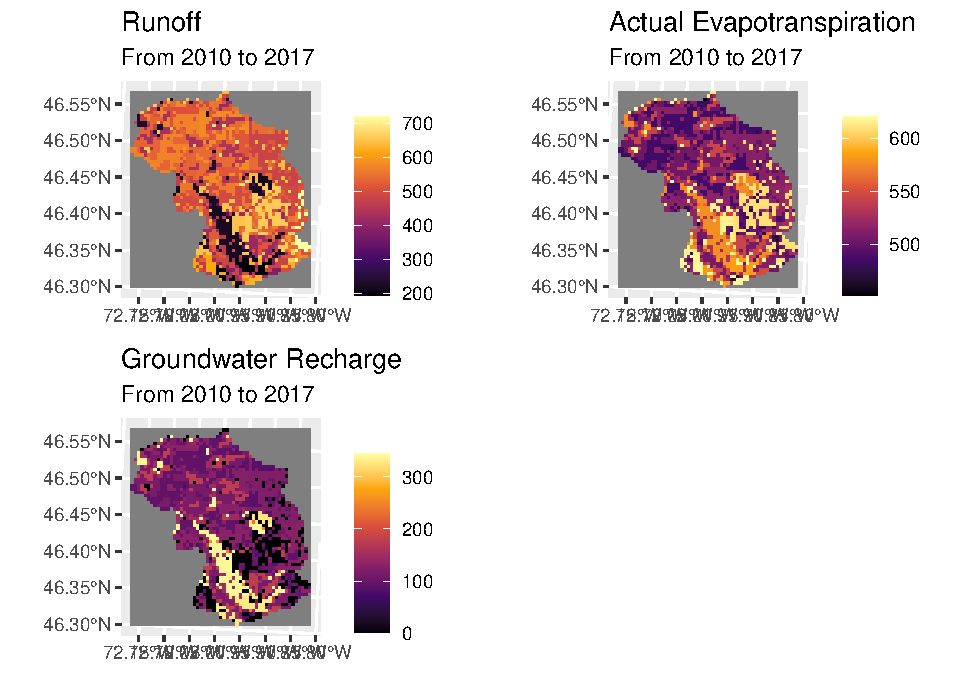
\includegraphics{fig/sim-viz-rasters-1.pdf}

\hypertarget{calibration-and-sensitity}{%
\chapter{Calibration and Sensitity}\label{calibration-and-sensitity}}

We will make use of \texttt{rechaRge} API to perform calibration and sensitivity analysis with different tools.

\hypertarget{quality-assessment}{%
\section{Quality assessment}\label{quality-assessment}}

Following the previous example, we will need to load observations datasets:

\begin{Shaded}
\begin{Highlighting}[]
\NormalTok{input\_rcn\_gauging }\OtherTok{\textless{}{-}} \FunctionTok{paste0}\NormalTok{(base\_url, }\StringTok{"rcn\_gauging.csv.gz"}\NormalTok{) }\CommentTok{\# relation between gaugins station and RCN cell IDs}
\NormalTok{input\_observed\_flow }\OtherTok{\textless{}{-}} \FunctionTok{paste0}\NormalTok{(base\_url, }\StringTok{"observed\_flow.csv.gz"}\NormalTok{) }\CommentTok{\# flow rates in mm/d}
\NormalTok{input\_alpha\_lyne\_hollick }\OtherTok{\textless{}{-}} \FunctionTok{paste0}\NormalTok{(base\_url, }\StringTok{"alpha\_lyne\_hollick.csv.gz"}\NormalTok{)}
\end{Highlighting}
\end{Shaded}

And we also need in this case to update the settings of the \textbf{HydroBudget} model object, so that column names match with the expected ones:

\begin{Shaded}
\begin{Highlighting}[]
\NormalTok{HB}\SpecialCharTok{$}\NormalTok{rcn\_gauging\_columns }\OtherTok{\textless{}{-}} \FunctionTok{list}\NormalTok{(}
  \AttributeTok{rcn\_id =} \StringTok{"cell\_ID"}\NormalTok{,}
  \AttributeTok{station\_id =} \StringTok{"gauging\_stat"}
\NormalTok{)}
\NormalTok{HB}\SpecialCharTok{$}\NormalTok{alpha\_lyne\_hollick\_columns}\SpecialCharTok{$}\NormalTok{station\_id }\OtherTok{\textless{}{-}} \StringTok{"station"}
\end{Highlighting}
\end{Shaded}

Then we can process the river flow observations and assess simulation quality:

\begin{Shaded}
\begin{Highlighting}[]
\NormalTok{quality }\OtherTok{\textless{}{-}}\NormalTok{ rechaRge}\SpecialCharTok{::}\FunctionTok{evaluate\_simulation\_quality}\NormalTok{(}
\NormalTok{  HB,}
  \AttributeTok{water\_budget =}\NormalTok{ water\_budget,}
  \AttributeTok{rcn\_gauging =}\NormalTok{ input\_rcn\_gauging,}
  \AttributeTok{observed\_flow =}\NormalTok{ input\_observed\_flow,}
  \AttributeTok{alpha\_lyne\_hollick =}\NormalTok{ input\_alpha\_lyne\_hollick,}
  \AttributeTok{period =}\NormalTok{ simul\_period}
\NormalTok{)}
\end{Highlighting}
\end{Shaded}

The \texttt{rechaRge} package proposes an model-free implementation of the \href{https://en.wikipedia.org/wiki/Kling\%E2\%80\%93Gupta_efficiency}{Kling-Gupta Efficiency} algorithm, that can be used for quality evaluation. In the case of our example the quality measurements of interest are:

\begin{Shaded}
\begin{Highlighting}[]
\FunctionTok{list}\NormalTok{(}
  \AttributeTok{KGE\_qtot\_cal\_mean =} \FunctionTok{mean}\NormalTok{(quality}\SpecialCharTok{$}\NormalTok{simulation\_metadata}\SpecialCharTok{$}\NormalTok{KGE\_qtot\_cal),}
  \AttributeTok{KGE\_qbase\_cal\_mean =} \FunctionTok{mean}\NormalTok{(quality}\SpecialCharTok{$}\NormalTok{simulation\_metadata}\SpecialCharTok{$}\NormalTok{KGE\_qbase\_cal))}
\end{Highlighting}
\end{Shaded}

\begin{verbatim}
$KGE_qtot_cal_mean
[1] 0.8549218

$KGE_qbase_cal_mean
[1] 0.7203224
\end{verbatim}

\hypertarget{using-sensitivity}{%
\section{Using sensitivity}\label{using-sensitivity}}

The \href{https://cran.r-project.org/package=sensitivity}{sensitivity} R package can perform various sensitivity analysis.

\hypertarget{define-model-function}{%
\subsection{Define model function}\label{define-model-function}}

\begin{Shaded}
\begin{Highlighting}[]
\FunctionTok{library}\NormalTok{(rechaRge)}
\FunctionTok{library}\NormalTok{(data.table)}

\CommentTok{\# Preload input data}
\CommentTok{\# Quiet download}
\FunctionTok{options}\NormalTok{(}\AttributeTok{datatable.showProgress =} \ConstantTok{FALSE}\NormalTok{)}
\CommentTok{\# use input example files provided by the package}
\NormalTok{base\_url }\OtherTok{\textless{}{-}} \StringTok{"https://github.com/gwrecharge/rechaRge{-}book/raw/main/examples/input/"}
\NormalTok{input\_rcn }\OtherTok{\textless{}{-}} \FunctionTok{fread}\NormalTok{(}\FunctionTok{paste0}\NormalTok{(base\_url, }\StringTok{"rcn.csv.gz"}\NormalTok{))}
\NormalTok{input\_climate }\OtherTok{\textless{}{-}} \FunctionTok{fread}\NormalTok{(}\FunctionTok{paste0}\NormalTok{(base\_url, }\StringTok{"climate.csv.gz"}\NormalTok{))}
\NormalTok{input\_rcn\_climate }\OtherTok{\textless{}{-}} \FunctionTok{fread}\NormalTok{(}\FunctionTok{paste0}\NormalTok{(base\_url, }\StringTok{"rcn\_climate.csv.gz"}\NormalTok{))}
\NormalTok{input\_rcn\_gauging }\OtherTok{\textless{}{-}} \FunctionTok{fread}\NormalTok{(}\FunctionTok{paste0}\NormalTok{(base\_url, }\StringTok{"rcn\_gauging.csv.gz"}\NormalTok{))}
\NormalTok{input\_observed\_flow }\OtherTok{\textless{}{-}} \FunctionTok{fread}\NormalTok{(}\FunctionTok{paste0}\NormalTok{(base\_url, }\StringTok{"observed\_flow.csv.gz"}\NormalTok{))}
\NormalTok{input\_alpha\_lyne\_hollick }\OtherTok{\textless{}{-}} \FunctionTok{fread}\NormalTok{(}\FunctionTok{paste0}\NormalTok{(base\_url, }\StringTok{"alpha\_lyne\_hollick.csv.gz"}\NormalTok{))}
\CommentTok{\# Simulation period}
\NormalTok{simul\_period }\OtherTok{\textless{}{-}} \FunctionTok{c}\NormalTok{(}\DecValTok{2017}\NormalTok{, }\DecValTok{2017}\NormalTok{)}

\NormalTok{hydrobudget\_eval }\OtherTok{\textless{}{-}} \ControlFlowTok{function}\NormalTok{(i) \{}
  \CommentTok{\# Calibration parameters}
\NormalTok{  HB }\OtherTok{\textless{}{-}}\NormalTok{ rechaRge}\SpecialCharTok{::}\FunctionTok{new\_hydrobudget}\NormalTok{(}
    \AttributeTok{T\_m =}\NormalTok{ i[}\DecValTok{1}\NormalTok{],}
    \CommentTok{\# melting temperature (°C)}
    \AttributeTok{C\_m =}\NormalTok{ i[}\DecValTok{2}\NormalTok{],}
    \CommentTok{\# melting coefficient (mm/°C/d)}
    \AttributeTok{TT\_F =}\NormalTok{ i[}\DecValTok{3}\NormalTok{],}
    \CommentTok{\# Threshold temperature for soil frost (°C)}
    \AttributeTok{F\_T =}\NormalTok{ i[}\DecValTok{4}\NormalTok{],}
    \CommentTok{\# Freezing time (d)}
    \AttributeTok{t\_API =}\NormalTok{ i[}\DecValTok{5}\NormalTok{],}
    \CommentTok{\# Antecedent precipitation index time (d)}
    \AttributeTok{f\_runoff =}\NormalTok{ i[}\DecValTok{6}\NormalTok{],}
    \CommentTok{\# Runoff factor ({-})}
    \AttributeTok{sw\_m =}\NormalTok{ i[}\DecValTok{7}\NormalTok{],}
    \CommentTok{\# Maximum soil water content (mm)}
    \AttributeTok{f\_inf =}\NormalTok{ i[}\DecValTok{8}\NormalTok{] }\CommentTok{\# infiltration factor ({-})}
\NormalTok{  )}
  \CommentTok{\# Input data specific settings}
\NormalTok{  HB}\SpecialCharTok{$}\NormalTok{rcn\_columns }\OtherTok{\textless{}{-}} \FunctionTok{list}\NormalTok{(}
    \AttributeTok{rcn\_id =} \StringTok{"cell\_ID"}\NormalTok{,}
    \AttributeTok{RCNII =} \StringTok{"RCNII"}\NormalTok{,}
    \AttributeTok{lon =} \StringTok{"X\_L93"}\NormalTok{,}
    \AttributeTok{lat =} \StringTok{"Y\_L93"}
\NormalTok{  )}
\NormalTok{  HB}\SpecialCharTok{$}\NormalTok{climate\_columns}\SpecialCharTok{$}\NormalTok{climate\_id }\OtherTok{\textless{}{-}} \StringTok{"climate\_cell"}
\NormalTok{  HB}\SpecialCharTok{$}\NormalTok{rcn\_climate\_columns }\OtherTok{\textless{}{-}} \FunctionTok{list}\NormalTok{(}\AttributeTok{climate\_id =} \StringTok{"climate\_cell"}\NormalTok{,}
                                 \AttributeTok{rcn\_id =} \StringTok{"cell\_ID"}\NormalTok{)}
\NormalTok{  HB}\SpecialCharTok{$}\NormalTok{rcn\_gauging\_columns }\OtherTok{\textless{}{-}} \FunctionTok{list}\NormalTok{(}\AttributeTok{rcn\_id =} \StringTok{"cell\_ID"}\NormalTok{,}
                                 \AttributeTok{station\_id =} \StringTok{"gauging\_stat"}\NormalTok{)}
\NormalTok{  HB}\SpecialCharTok{$}\NormalTok{alpha\_lyne\_hollick\_columns}\SpecialCharTok{$}\NormalTok{station\_id }\OtherTok{\textless{}{-}} \StringTok{"station"}

  \CommentTok{\# Simulation with the HydroBudget model}
\NormalTok{  water\_budget }\OtherTok{\textless{}{-}}\NormalTok{ rechaRge}\SpecialCharTok{::}\FunctionTok{compute\_recharge}\NormalTok{(}
\NormalTok{    HB,}
    \AttributeTok{rcn =}\NormalTok{ input\_rcn,}
    \AttributeTok{climate =}\NormalTok{ input\_climate,}
    \AttributeTok{rcn\_climate =}\NormalTok{ input\_rcn\_climate,}
    \AttributeTok{period =}\NormalTok{ simul\_period,}
    \AttributeTok{workers =} \DecValTok{1}
\NormalTok{  )}

  \CommentTok{\# Evaluate simulation quality}
\NormalTok{  result }\OtherTok{\textless{}{-}}\NormalTok{ rechaRge}\SpecialCharTok{::}\FunctionTok{evaluate\_simulation\_quality}\NormalTok{(}
\NormalTok{    HB,}
    \AttributeTok{water\_budget =}\NormalTok{ water\_budget,}
    \AttributeTok{rcn\_gauging =}\NormalTok{ input\_rcn\_gauging,}
    \AttributeTok{observed\_flow =}\NormalTok{ input\_observed\_flow,}
    \AttributeTok{alpha\_lyne\_hollick =}\NormalTok{ input\_alpha\_lyne\_hollick,}
    \AttributeTok{period =}\NormalTok{ simul\_period}
\NormalTok{  )}

  \FunctionTok{return}\NormalTok{(}\FunctionTok{c}\NormalTok{(}
    \FunctionTok{mean}\NormalTok{(result}\SpecialCharTok{$}\NormalTok{simulation\_metadata}\SpecialCharTok{$}\NormalTok{KGE\_qtot\_cal),}
    \FunctionTok{mean}\NormalTok{(result}\SpecialCharTok{$}\NormalTok{simulation\_metadata}\SpecialCharTok{$}\NormalTok{KGE\_qbase\_cal)}
\NormalTok{  ))}
\NormalTok{\}}
\end{Highlighting}
\end{Shaded}

\hypertarget{run-sensitivity-analysis}{%
\subsection{Run sensitivity analysis}\label{run-sensitivity-analysis}}

\begin{Shaded}
\begin{Highlighting}[]
\FunctionTok{library}\NormalTok{(sensitivity)}
\CommentTok{\# Use future package to parallel}
\FunctionTok{library}\NormalTok{(future.apply)}

\NormalTok{hydrobudget\_sens }\OtherTok{\textless{}{-}} \ControlFlowTok{function}\NormalTok{(X) \{}
\NormalTok{  kge\_hb }\OtherTok{\textless{}{-}} \FunctionTok{as.matrix}\NormalTok{(}\FunctionTok{t}\NormalTok{(}\FunctionTok{future\_apply}\NormalTok{(X, }\AttributeTok{MARGIN =} \DecValTok{1}\NormalTok{, }\AttributeTok{FUN =}\NormalTok{ hydrobudget\_eval, }\AttributeTok{future.seed =} \ConstantTok{TRUE}\NormalTok{)))}
  \FunctionTok{return}\NormalTok{(kge\_hb)}
\NormalTok{\}}

\CommentTok{\# Number of variables}
\NormalTok{nvar }\OtherTok{\textless{}{-}} \DecValTok{8}
\CommentTok{\# Range of the parameters}
\NormalTok{binf }\OtherTok{\textless{}{-}} \FunctionTok{c}\NormalTok{(}\DecValTok{1}\NormalTok{, }\DecValTok{4}\NormalTok{, }\SpecialCharTok{{-}}\DecValTok{20}\NormalTok{, }\DecValTok{5}\NormalTok{, }\FloatTok{3.05}\NormalTok{, }\FloatTok{0.5}\NormalTok{, }\DecValTok{160}\NormalTok{, }\FloatTok{0.01}\NormalTok{)}
\NormalTok{bsup }\OtherTok{\textless{}{-}} \FunctionTok{c}\NormalTok{(}\FloatTok{2.5}\NormalTok{, }\FloatTok{6.5}\NormalTok{, }\SpecialCharTok{{-}}\DecValTok{12}\NormalTok{, }\DecValTok{30}\NormalTok{, }\FloatTok{4.8}\NormalTok{, }\FloatTok{0.6}\NormalTok{, }\DecValTok{720}\NormalTok{, }\FloatTok{0.05}\NormalTok{)}

\CommentTok{\# parallel computation setting}
\FunctionTok{plan}\NormalTok{(multisession, }\AttributeTok{workers =} \DecValTok{3}\NormalTok{)}
\CommentTok{\#plan(sequential) \# non parallel}
\NormalTok{sensitivity\_results }\OtherTok{\textless{}{-}} \FunctionTok{morris}\NormalTok{(}
  \AttributeTok{model =}\NormalTok{ hydrobudget\_sens,}
  \AttributeTok{factors =}\NormalTok{ nvar,}
  \AttributeTok{r =} \DecValTok{2}\NormalTok{,}
  \AttributeTok{design =} \FunctionTok{list}\NormalTok{(}\AttributeTok{type =} \StringTok{"oat"}\NormalTok{, }\AttributeTok{levels =} \DecValTok{5}\NormalTok{, }\AttributeTok{grid.jump =} \DecValTok{3}\NormalTok{),}
  \AttributeTok{binf =}\NormalTok{ binf,}
  \AttributeTok{bsup =}\NormalTok{ bsup)}
\end{Highlighting}
\end{Shaded}

\hypertarget{handle-sensitivity-results}{%
\subsection{Handle sensitivity results}\label{handle-sensitivity-results}}

\begin{Shaded}
\begin{Highlighting}[]
\CommentTok{\# Variable of interest}
\NormalTok{mu }\OtherTok{\textless{}{-}} \FunctionTok{apply}\NormalTok{(sensitivity\_results}\SpecialCharTok{$}\NormalTok{ee, }\DecValTok{3}\NormalTok{, }\ControlFlowTok{function}\NormalTok{(M)\{}
  \FunctionTok{apply}\NormalTok{(M, }\DecValTok{2}\NormalTok{, mean)}
\NormalTok{\})}
\NormalTok{mu.star }\OtherTok{\textless{}{-}} \FunctionTok{apply}\NormalTok{(}\FunctionTok{abs}\NormalTok{(sensitivity\_results}\SpecialCharTok{$}\NormalTok{ee), }\DecValTok{3}\NormalTok{, }\ControlFlowTok{function}\NormalTok{(M)\{}
  \FunctionTok{apply}\NormalTok{(M, }\DecValTok{2}\NormalTok{, mean)}
\NormalTok{\})}
\NormalTok{sigma }\OtherTok{\textless{}{-}} \FunctionTok{apply}\NormalTok{(sensitivity\_results}\SpecialCharTok{$}\NormalTok{ee, }\DecValTok{3}\NormalTok{, }\ControlFlowTok{function}\NormalTok{(M)\{}
  \FunctionTok{apply}\NormalTok{(M, }\DecValTok{2}\NormalTok{, sd)}
\NormalTok{\})}
\NormalTok{sensitivity\_eval }\OtherTok{\textless{}{-}} \FunctionTok{data.table}\NormalTok{(}\AttributeTok{mu =}\NormalTok{ mu, }\AttributeTok{mu.star =}\NormalTok{ mu.star, }\AttributeTok{sigma =}\NormalTok{ sigma)}
\end{Highlighting}
\end{Shaded}

\begin{tabular}{r|r|r|r|r|r}
\hline
mu.ycol1 & mu.ycol2 & mu.star.ycol1 & mu.star.ycol2 & sigma.ycol1 & sigma.ycol2\\
\hline
0.1258523 & -0.0366606 & 0.1258523 & 0.0386035 & 0.0118168 & 0.0545936\\
\hline
-0.0167993 & 0.0721534 & 0.0167993 & 0.0721534 & 0.0208969 & 0.0364881\\
\hline
-0.0004497 & -0.0024241 & 0.0004497 & 0.0024241 & 0.0006359 & 0.0034282\\
\hline
0.0000000 & 0.0000000 & 0.0000000 & 0.0000000 & 0.0000000 & 0.0000000\\
\hline
0.0161598 & 0.0192713 & 0.0161598 & 0.0276047 & 0.0073267 & 0.0390389\\
\hline
0.0375014 & -0.0405481 & 0.0375014 & 0.0454711 & 0.0278842 & 0.0643059\\
\hline
-0.4140280 & -0.4979411 & 0.4140280 & 0.4979411 & 0.0275821 & 0.2715614\\
\hline
0.0741573 & 0.1943334 & 0.0741573 & 0.6462617 & 0.0585579 & 0.9139521\\
\hline
\end{tabular}

\begin{Shaded}
\begin{Highlighting}[]
\CommentTok{\# Plot}
\FunctionTok{plot}\NormalTok{(sensitivity\_results, }\AttributeTok{y\_col =} \DecValTok{2}\NormalTok{)}
\FunctionTok{title}\NormalTok{(}\AttributeTok{main =} \StringTok{"y\_col = 2"}\NormalTok{)}
\end{Highlighting}
\end{Shaded}

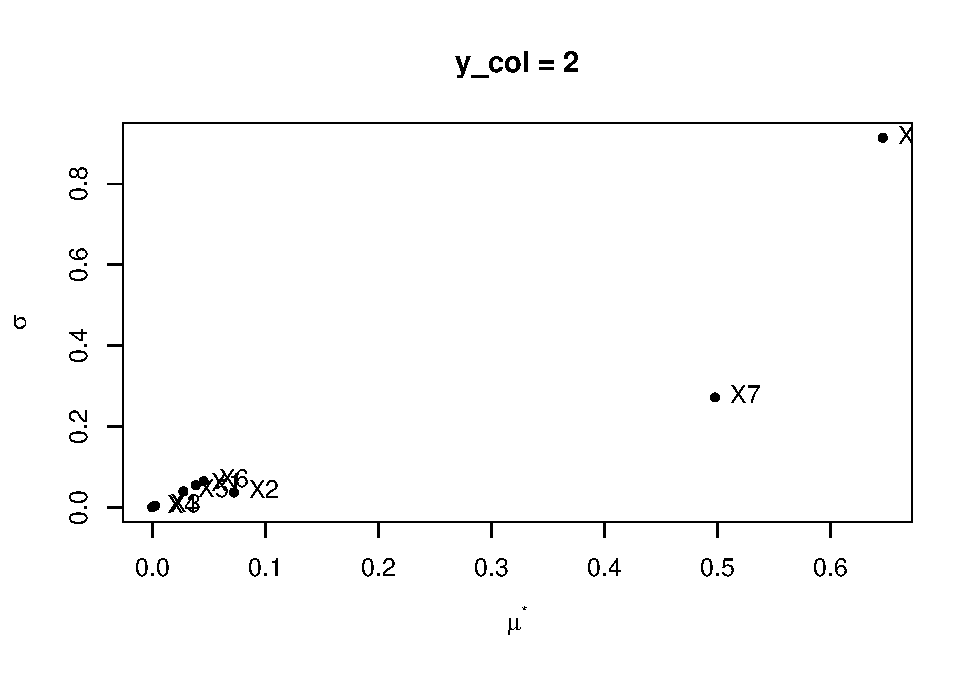
\includegraphics{fig/unnamed-chunk-3-1.pdf}

\begin{Shaded}
\begin{Highlighting}[]
\FunctionTok{plot.new}\NormalTok{()}
\FunctionTok{plot}\NormalTok{(sensitivity\_results, }\AttributeTok{y\_col =} \DecValTok{1}\NormalTok{)}
\FunctionTok{title}\NormalTok{(}\AttributeTok{main =} \StringTok{"y\_col = 1"}\NormalTok{)}
\end{Highlighting}
\end{Shaded}

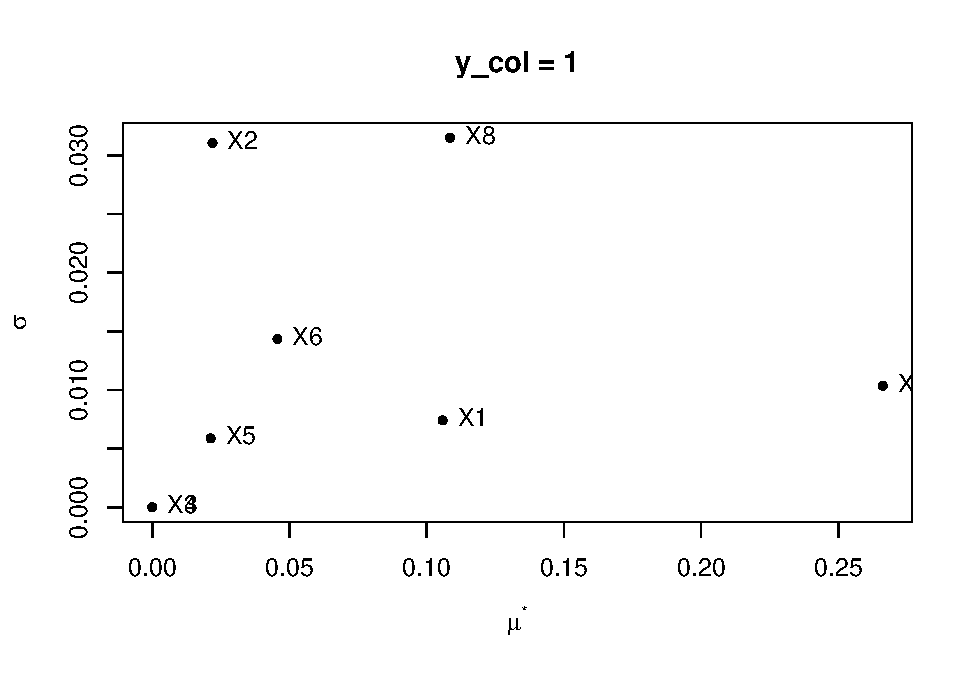
\includegraphics{fig/unnamed-chunk-4-1.pdf}

\hypertarget{using-caramel}{%
\section{Using caRamel}\label{using-caramel}}

The \href{https://cran.r-project.org/package=caRamel}{caRamel} R package can perform both calibration and sensitivity analysis.

\hypertarget{define-objective-function}{%
\subsection{Define objective function}\label{define-objective-function}}

We will start by defining the objective function to optimize: this function will run a simulation and quality evaluation and its returned values will be used by \texttt{caRamel} to measure the quality of the injected parameters.

\begin{Shaded}
\begin{Highlighting}[]
\NormalTok{make\_hydrobudget\_eval }\OtherTok{\textless{}{-}} \ControlFlowTok{function}\NormalTok{() \{}
  \CommentTok{\# Preload input data}
  \CommentTok{\# Quiet download}
  \FunctionTok{options}\NormalTok{(}\AttributeTok{datatable.showProgress =} \ConstantTok{FALSE}\NormalTok{)}
  \CommentTok{\# use input example files provided by the package}
\NormalTok{  base\_url }\OtherTok{\textless{}{-}} \StringTok{"https://github.com/gwrecharge/rechaRge{-}book/raw/main/examples/input/"}
\NormalTok{  input\_rcn }\OtherTok{\textless{}{-}} \FunctionTok{fread}\NormalTok{(}\FunctionTok{paste0}\NormalTok{(base\_url, }\StringTok{"rcn.csv.gz"}\NormalTok{))}
\NormalTok{  input\_climate }\OtherTok{\textless{}{-}} \FunctionTok{fread}\NormalTok{(}\FunctionTok{paste0}\NormalTok{(base\_url, }\StringTok{"climate.csv.gz"}\NormalTok{))}
\NormalTok{  input\_rcn\_climate }\OtherTok{\textless{}{-}} \FunctionTok{fread}\NormalTok{(}\FunctionTok{paste0}\NormalTok{(base\_url, }\StringTok{"rcn\_climate.csv.gz"}\NormalTok{))}
\NormalTok{  input\_rcn\_gauging }\OtherTok{\textless{}{-}} \FunctionTok{fread}\NormalTok{(}\FunctionTok{paste0}\NormalTok{(base\_url, }\StringTok{"rcn\_gauging.csv.gz"}\NormalTok{))}
\NormalTok{  input\_observed\_flow }\OtherTok{\textless{}{-}} \FunctionTok{fread}\NormalTok{(}\FunctionTok{paste0}\NormalTok{(base\_url, }\StringTok{"observed\_flow.csv.gz"}\NormalTok{))}
\NormalTok{  input\_alpha\_lyne\_hollick }\OtherTok{\textless{}{-}} \FunctionTok{fread}\NormalTok{(}\FunctionTok{paste0}\NormalTok{(base\_url, }\StringTok{"alpha\_lyne\_hollick.csv.gz"}\NormalTok{))}
  \CommentTok{\# Simulation period}
\NormalTok{  simul\_period }\OtherTok{\textless{}{-}} \FunctionTok{c}\NormalTok{(}\DecValTok{2017}\NormalTok{, }\DecValTok{2017}\NormalTok{)}

\NormalTok{  hydrobudget\_eval }\OtherTok{\textless{}{-}} \ControlFlowTok{function}\NormalTok{(i) \{}
    \CommentTok{\# Calibration parameters}
\NormalTok{    HB }\OtherTok{\textless{}{-}}\NormalTok{ rechaRge}\SpecialCharTok{::}\FunctionTok{new\_hydrobudget}\NormalTok{(}
      \AttributeTok{T\_m =}\NormalTok{ x[i, }\DecValTok{1}\NormalTok{],}
      \CommentTok{\# melting temperature (°C)}
      \AttributeTok{C\_m =}\NormalTok{ x[i, }\DecValTok{2}\NormalTok{],}
      \CommentTok{\# melting coefficient (mm/°C/d)}
      \AttributeTok{TT\_F =}\NormalTok{ x[i, }\DecValTok{3}\NormalTok{],}
      \CommentTok{\# Threshold temperature for soil frost (°C)}
      \AttributeTok{F\_T =}\NormalTok{ x[i, }\DecValTok{4}\NormalTok{],}
      \CommentTok{\# Freezing time (d)}
      \AttributeTok{t\_API =}\NormalTok{ x[i, }\DecValTok{5}\NormalTok{],}
      \CommentTok{\# Antecedent precipitation index time (d)}
      \AttributeTok{f\_runoff =}\NormalTok{ x[i, }\DecValTok{6}\NormalTok{],}
      \CommentTok{\# Runoff factor ({-})}
      \AttributeTok{sw\_m =}\NormalTok{ x[i, }\DecValTok{7}\NormalTok{],}
      \CommentTok{\# Maximum soil water content (mm)}
      \AttributeTok{f\_inf =}\NormalTok{ x[i, }\DecValTok{8}\NormalTok{] }\CommentTok{\# infiltration factor ({-})}
\NormalTok{    )}
    \CommentTok{\# Input data specific settings}
\NormalTok{    HB}\SpecialCharTok{$}\NormalTok{rcn\_columns }\OtherTok{\textless{}{-}} \FunctionTok{list}\NormalTok{(}
      \AttributeTok{rcn\_id =} \StringTok{"cell\_ID"}\NormalTok{,}
      \AttributeTok{RCNII =} \StringTok{"RCNII"}\NormalTok{,}
      \AttributeTok{lon =} \StringTok{"X\_L93"}\NormalTok{,}
      \AttributeTok{lat =} \StringTok{"Y\_L93"}
\NormalTok{    )}
\NormalTok{    HB}\SpecialCharTok{$}\NormalTok{climate\_columns}\SpecialCharTok{$}\NormalTok{climate\_id }\OtherTok{\textless{}{-}} \StringTok{"climate\_cell"}
\NormalTok{    HB}\SpecialCharTok{$}\NormalTok{rcn\_climate\_columns }\OtherTok{\textless{}{-}} \FunctionTok{list}\NormalTok{(}\AttributeTok{climate\_id =} \StringTok{"climate\_cell"}\NormalTok{,}
                                   \AttributeTok{rcn\_id =} \StringTok{"cell\_ID"}\NormalTok{)}
\NormalTok{    HB}\SpecialCharTok{$}\NormalTok{rcn\_gauging\_columns }\OtherTok{\textless{}{-}} \FunctionTok{list}\NormalTok{(}\AttributeTok{rcn\_id =} \StringTok{"cell\_ID"}\NormalTok{,}
                                   \AttributeTok{station\_id =} \StringTok{"gauging\_stat"}\NormalTok{)}
\NormalTok{    HB}\SpecialCharTok{$}\NormalTok{alpha\_lyne\_hollick\_columns}\SpecialCharTok{$}\NormalTok{station\_id }\OtherTok{\textless{}{-}} \StringTok{"station"}

    \CommentTok{\# Simulation with the HydroBudget model}
\NormalTok{    rechaRge}\SpecialCharTok{::}\FunctionTok{with\_verbose}\NormalTok{(}\ConstantTok{FALSE}\NormalTok{)}
\NormalTok{    water\_budget }\OtherTok{\textless{}{-}}\NormalTok{ rechaRge}\SpecialCharTok{::}\FunctionTok{compute\_recharge}\NormalTok{(}
\NormalTok{      HB,}
      \AttributeTok{rcn =}\NormalTok{ input\_rcn,}
      \AttributeTok{climate =}\NormalTok{ input\_climate,}
      \AttributeTok{rcn\_climate =}\NormalTok{ input\_rcn\_climate,}
      \AttributeTok{period =}\NormalTok{ simul\_period,}
      \AttributeTok{workers =} \DecValTok{1} \CommentTok{\# do not parallelize, caRamel will do it}
\NormalTok{    )}

    \CommentTok{\# Evaluate simulation quality}
\NormalTok{    quality }\OtherTok{\textless{}{-}}\NormalTok{ rechaRge}\SpecialCharTok{::}\FunctionTok{evaluate\_simulation\_quality}\NormalTok{(}
\NormalTok{      HB,}
      \AttributeTok{water\_budget =}\NormalTok{ water\_budget,}
      \AttributeTok{rcn\_gauging =}\NormalTok{ input\_rcn\_gauging,}
      \AttributeTok{observed\_flow =}\NormalTok{ input\_observed\_flow,}
      \AttributeTok{alpha\_lyne\_hollick =}\NormalTok{ input\_alpha\_lyne\_hollick,}
      \AttributeTok{period =}\NormalTok{ simul\_period}
\NormalTok{    )}

    \FunctionTok{return}\NormalTok{(}\FunctionTok{c}\NormalTok{(}
      \FunctionTok{mean}\NormalTok{(quality}\SpecialCharTok{$}\NormalTok{simulation\_metadata}\SpecialCharTok{$}\NormalTok{KGE\_qtot\_cal),}
      \FunctionTok{mean}\NormalTok{(quality}\SpecialCharTok{$}\NormalTok{simulation\_metadata}\SpecialCharTok{$}\NormalTok{KGE\_qbase\_cal)}
\NormalTok{    ))}
\NormalTok{  \}}

  \FunctionTok{return}\NormalTok{(hydrobudget\_eval)}
\NormalTok{\}}
\end{Highlighting}
\end{Shaded}

\hypertarget{run-calibration-analysis}{%
\subsection{Run calibration analysis}\label{run-calibration-analysis}}

Then perform calibration with sensitivity:

\begin{Shaded}
\begin{Highlighting}[]
\FunctionTok{library}\NormalTok{(caRamel)}

\CommentTok{\# Number of objectives}
\NormalTok{nobj }\OtherTok{\textless{}{-}} \DecValTok{2}
\CommentTok{\# Number of variables}
\NormalTok{nvar }\OtherTok{\textless{}{-}} \DecValTok{8}
\CommentTok{\# All the objectives are to be maximized}
\NormalTok{minmax }\OtherTok{\textless{}{-}} \FunctionTok{c}\NormalTok{(}\ConstantTok{TRUE}\NormalTok{, }\ConstantTok{TRUE}\NormalTok{)}
\CommentTok{\# Ranges of the parameters}
\NormalTok{bounds }\OtherTok{\textless{}{-}} \FunctionTok{matrix}\NormalTok{(}\AttributeTok{nrow =}\NormalTok{ nvar, }\AttributeTok{ncol =} \DecValTok{2}\NormalTok{)}
\NormalTok{bounds[, }\DecValTok{1}\NormalTok{] }\OtherTok{\textless{}{-}} \FunctionTok{c}\NormalTok{(}\DecValTok{1}\NormalTok{, }\DecValTok{4}\NormalTok{, }\SpecialCharTok{{-}}\DecValTok{20}\NormalTok{, }\DecValTok{5}\NormalTok{, }\FloatTok{3.05}\NormalTok{, }\FloatTok{0.5}\NormalTok{, }\DecValTok{160}\NormalTok{, }\FloatTok{0.01}\NormalTok{)}
\NormalTok{bounds[, }\DecValTok{2}\NormalTok{] }\OtherTok{\textless{}{-}} \FunctionTok{c}\NormalTok{(}\FloatTok{2.5}\NormalTok{, }\FloatTok{6.5}\NormalTok{, }\SpecialCharTok{{-}}\DecValTok{12}\NormalTok{, }\DecValTok{30}\NormalTok{, }\FloatTok{4.8}\NormalTok{, }\FloatTok{0.6}\NormalTok{, }\DecValTok{720}\NormalTok{, }\FloatTok{0.05}\NormalTok{)}

\NormalTok{calibration\_results }\OtherTok{\textless{}{-}} \FunctionTok{caRamel}\NormalTok{(}
  \AttributeTok{nobj =}\NormalTok{ nobj,}
  \AttributeTok{nvar =}\NormalTok{ nvar,}
  \AttributeTok{minmax =}\NormalTok{  minmax,}
  \AttributeTok{bounds =}\NormalTok{ bounds,}
  \AttributeTok{func =} \FunctionTok{make\_hydrobudget\_eval}\NormalTok{(),}
  \AttributeTok{prec =} \FunctionTok{matrix}\NormalTok{(}\FloatTok{0.01}\NormalTok{, }\AttributeTok{nrow =} \DecValTok{1}\NormalTok{, }\AttributeTok{ncol =}\NormalTok{ nobj),}
  \AttributeTok{sensitivity =} \ConstantTok{FALSE}\NormalTok{, }\CommentTok{\# you can include sensitivity analysis}
  \AttributeTok{archsize =} \DecValTok{100}\NormalTok{,}\CommentTok{\# adjust to relevant value}
  \AttributeTok{popsize =} \DecValTok{10}\NormalTok{,  }\CommentTok{\# adjust to relevant value}
  \AttributeTok{maxrun =} \DecValTok{10}\NormalTok{,   }\CommentTok{\# adjust to relevant value}
  \AttributeTok{carallel =} \DecValTok{1}\NormalTok{, }\CommentTok{\# do parallel ...}
  \AttributeTok{numcores =} \DecValTok{2}  \CommentTok{\# ... on 2 cores}
\NormalTok{)}
\end{Highlighting}
\end{Shaded}

\hypertarget{handle-calibration-results}{%
\subsection{Handle calibration results}\label{handle-calibration-results}}

Make use of calibration results, by merging simulation outputs with front objectives, to get more readable parameters, ordered by ``best fit'' score:

\begin{Shaded}
\begin{Highlighting}[]
\NormalTok{output\_front }\OtherTok{\textless{}{-}} \FunctionTok{data.table}\NormalTok{(}\FunctionTok{cbind}\NormalTok{(calibration\_results}\SpecialCharTok{$}\NormalTok{parameters, calibration\_results}\SpecialCharTok{$}\NormalTok{objectives))}
\FunctionTok{colnames}\NormalTok{(output\_front) }\OtherTok{\textless{}{-}} \FunctionTok{c}\NormalTok{(}\StringTok{"T\_m"}\NormalTok{, }\StringTok{"C\_m"}\NormalTok{, }\StringTok{"TT\_F"}\NormalTok{, }\StringTok{"F\_T"}\NormalTok{, }\StringTok{"t\_API"}\NormalTok{, }\StringTok{"f\_runoff"}\NormalTok{, }\StringTok{"sw\_m"}\NormalTok{, }\StringTok{"f\_inf"}\NormalTok{, }\StringTok{"KGE\_qtot"}\NormalTok{, }\StringTok{"KGE\_qbase"}\NormalTok{)}
\NormalTok{y }\OtherTok{\textless{}{-}} \FloatTok{0.6} \CommentTok{\# choose your KGE weight criteria}
\NormalTok{output\_front[, }\StringTok{\textasciigrave{}}\AttributeTok{:=}\StringTok{\textasciigrave{}}\NormalTok{(}\AttributeTok{KGE\_score =}\NormalTok{ (KGE\_qtot }\SpecialCharTok{*}\NormalTok{ (}\DecValTok{1} \SpecialCharTok{{-}}\NormalTok{ y) }\SpecialCharTok{+}\NormalTok{ KGE\_qbase }\SpecialCharTok{*}\NormalTok{ y))]}
\NormalTok{output\_front }\OtherTok{\textless{}{-}}\NormalTok{ output\_front[}\FunctionTok{order}\NormalTok{(KGE\_score, }\AttributeTok{decreasing =} \ConstantTok{TRUE}\NormalTok{)]}
\end{Highlighting}
\end{Shaded}

\begin{tabular}{r|r|r|r|r|r|r|r|r|r|r}
\hline
T\_m & C\_m & TT\_F & F\_T & t\_API & f\_runoff & sw\_m & f\_inf & KGE\_qtot & KGE\_qbase & KGE\_score\\
\hline
1.679990 & 4.223536 & -12.73111 & 11.17360 & 4.737293 & 0.5861675 & 160.9877 & 0.0353507 & 0.7273544 & 0.7130841 & 0.7187922\\
\hline
1.085446 & 6.196717 & -13.59741 & 28.86741 & 3.402038 & 0.5901827 & 319.5927 & 0.0413703 & 0.4950154 & 0.8204889 & 0.6902995\\
\hline
2.389945 & 5.356833 & -14.60400 & 23.79462 & 4.543765 & 0.5137648 & 265.5619 & 0.0322331 & 0.6310661 & 0.7133485 & 0.6804355\\
\hline
\end{tabular}

Display the results with \texttt{caRamel}'s plotting feature:

\begin{Shaded}
\begin{Highlighting}[]
\CommentTok{\# Plot using caRamel}
\FunctionTok{plot\_caramel}\NormalTok{(calibration\_results, }\AttributeTok{objnames =} \FunctionTok{c}\NormalTok{(}\StringTok{"KGE\_qtot"}\NormalTok{, }\StringTok{"KGE\_qbase"}\NormalTok{))}
\end{Highlighting}
\end{Shaded}

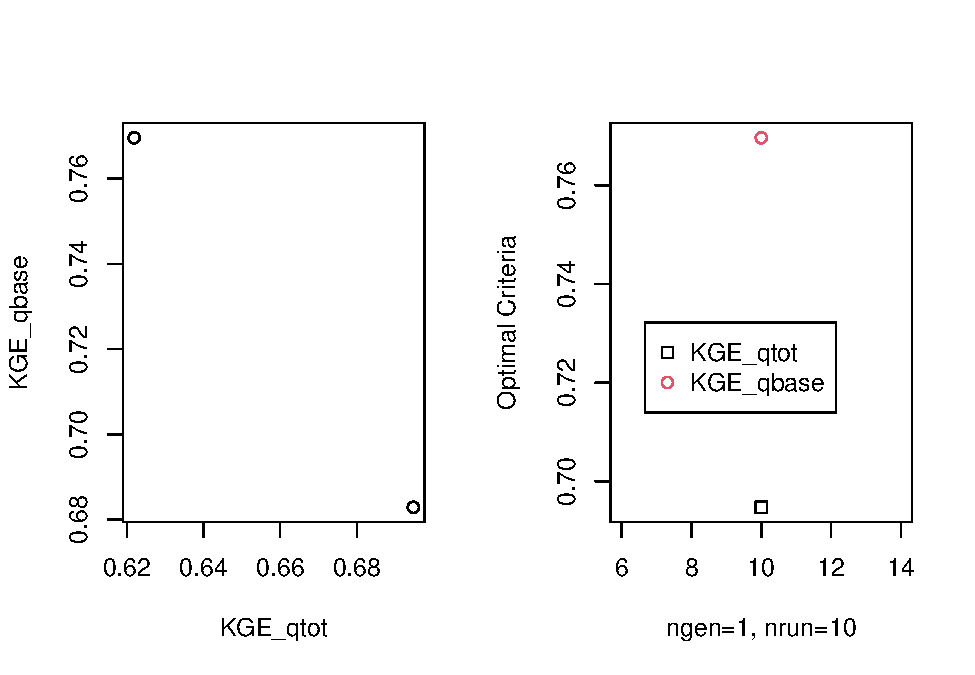
\includegraphics{fig/unnamed-chunk-6-1.pdf}

Scatter plot the calibration's simulations, with the resulting \href{https://en.wikipedia.org/wiki/Pareto_front}{Pareto front}:

\begin{Shaded}
\begin{Highlighting}[]
\CommentTok{\# Plot all using ggplot}
\FunctionTok{library}\NormalTok{(ggplot2)}
\NormalTok{front }\OtherTok{\textless{}{-}} \FunctionTok{data.table}\NormalTok{(calibration\_results}\SpecialCharTok{$}\NormalTok{objectives)}
\FunctionTok{colnames}\NormalTok{(front) }\OtherTok{\textless{}{-}} \FunctionTok{c}\NormalTok{(}\StringTok{"KGE\_qtot"}\NormalTok{, }\StringTok{"KGE\_qbase"}\NormalTok{)}
\NormalTok{all }\OtherTok{\textless{}{-}} \FunctionTok{data.table}\NormalTok{(calibration\_results}\SpecialCharTok{$}\NormalTok{total\_pop[, }\DecValTok{9}\SpecialCharTok{:}\DecValTok{10}\NormalTok{])}
\FunctionTok{colnames}\NormalTok{(all) }\OtherTok{\textless{}{-}} \FunctionTok{c}\NormalTok{(}\StringTok{"KGE\_qtot"}\NormalTok{, }\StringTok{"KGE\_qbase"}\NormalTok{)}
\NormalTok{combined\_data }\OtherTok{\textless{}{-}} \FunctionTok{rbind}\NormalTok{(all, front)}
\NormalTok{combined\_data}\SpecialCharTok{$}\NormalTok{group }\OtherTok{\textless{}{-}} \FunctionTok{c}\NormalTok{(}\FunctionTok{rep}\NormalTok{(}\StringTok{"All"}\NormalTok{, }\FunctionTok{nrow}\NormalTok{(all)), }\FunctionTok{rep}\NormalTok{(}\StringTok{"Front"}\NormalTok{, }\FunctionTok{nrow}\NormalTok{(front)))}
\FunctionTok{ggplot}\NormalTok{(combined\_data, }\FunctionTok{aes}\NormalTok{(}\AttributeTok{x =}\NormalTok{ KGE\_qtot, }\AttributeTok{y =}\NormalTok{ KGE\_qbase, }\AttributeTok{color =}\NormalTok{ group)) }\SpecialCharTok{+}
  \FunctionTok{geom\_point}\NormalTok{() }\SpecialCharTok{+}
  \FunctionTok{labs}\NormalTok{(}\AttributeTok{title =} \StringTok{"Scatter plot of simulations"}\NormalTok{,}
       \AttributeTok{x =} \StringTok{"KGE\_qtot"}\NormalTok{, }\AttributeTok{y =} \StringTok{"KGE\_qbase"}\NormalTok{,}
       \AttributeTok{color =} \StringTok{"Dataset"}\NormalTok{) }\SpecialCharTok{+}
  \FunctionTok{theme\_minimal}\NormalTok{()}
\end{Highlighting}
\end{Shaded}

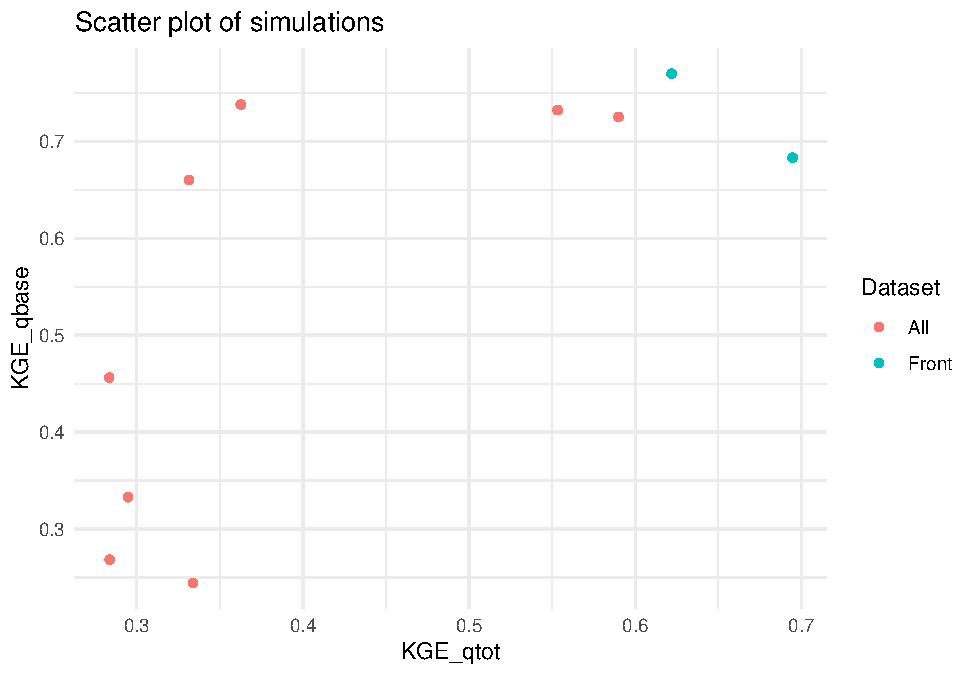
\includegraphics{fig/calib-crml-scatter-plot-1.pdf}

\hypertarget{evaluate-uncertainty}{%
\subsection{Evaluate uncertainty}\label{evaluate-uncertainty}}

For each set of parameters proposed by \texttt{caRamel}, run a simulation and then evaluate the uncertainty of the set of parameters identified as being the ``best fit''.

\begin{Shaded}
\begin{Highlighting}[]
\CommentTok{\# for each proposed set of parameters, run the water budget simulation}
\NormalTok{param\_ids }\OtherTok{\textless{}{-}} \FunctionTok{as.numeric}\NormalTok{(}\FunctionTok{rownames}\NormalTok{(output\_front))}

\CommentTok{\# run simulations}
\NormalTok{water\_budgets }\OtherTok{\textless{}{-}} \FunctionTok{lapply}\NormalTok{(param\_ids, }\AttributeTok{FUN =} \ControlFlowTok{function}\NormalTok{(i) \{}
\NormalTok{  x }\OtherTok{\textless{}{-}}\NormalTok{ output\_front}
\NormalTok{  HB }\OtherTok{\textless{}{-}}\NormalTok{ rechaRge}\SpecialCharTok{::}\FunctionTok{new\_hydrobudget}\NormalTok{(}
    \AttributeTok{T\_m =} \FunctionTok{as.numeric}\NormalTok{(x[i, }\DecValTok{1}\NormalTok{]),}
    \AttributeTok{C\_m =} \FunctionTok{as.numeric}\NormalTok{(x[i, }\DecValTok{2}\NormalTok{]),}
    \AttributeTok{TT\_F =} \FunctionTok{as.numeric}\NormalTok{(x[i, }\DecValTok{3}\NormalTok{]),}
    \AttributeTok{F\_T =} \FunctionTok{as.numeric}\NormalTok{(x[i, }\DecValTok{4}\NormalTok{]),}
    \AttributeTok{t\_API =} \FunctionTok{as.numeric}\NormalTok{(x[i, }\DecValTok{5}\NormalTok{]),}
    \AttributeTok{f\_runoff =} \FunctionTok{as.numeric}\NormalTok{(x[i, }\DecValTok{6}\NormalTok{]),}
    \AttributeTok{sw\_m =} \FunctionTok{as.numeric}\NormalTok{(x[i, }\DecValTok{7}\NormalTok{]),}
    \AttributeTok{f\_inf =} \FunctionTok{as.numeric}\NormalTok{(x[i, }\DecValTok{8}\NormalTok{])}
\NormalTok{  )}
  \CommentTok{\# Input data specific settings}
\NormalTok{  HB}\SpecialCharTok{$}\NormalTok{rcn\_columns }\OtherTok{\textless{}{-}} \FunctionTok{list}\NormalTok{(}
    \AttributeTok{rcn\_id =} \StringTok{"cell\_ID"}\NormalTok{,}
    \AttributeTok{RCNII =} \StringTok{"RCNII"}\NormalTok{,}
    \AttributeTok{lon =} \StringTok{"X\_L93"}\NormalTok{,}
    \AttributeTok{lat =} \StringTok{"Y\_L93"}
\NormalTok{  )}
\NormalTok{  HB}\SpecialCharTok{$}\NormalTok{climate\_columns}\SpecialCharTok{$}\NormalTok{climate\_id }\OtherTok{\textless{}{-}} \StringTok{"climate\_cell"}
\NormalTok{  HB}\SpecialCharTok{$}\NormalTok{rcn\_climate\_columns }\OtherTok{\textless{}{-}} \FunctionTok{list}\NormalTok{(}\AttributeTok{climate\_id =} \StringTok{"climate\_cell"}\NormalTok{,}
                                 \AttributeTok{rcn\_id =} \StringTok{"cell\_ID"}\NormalTok{)}

  \CommentTok{\# Simulation with the HydroBudget model}
\NormalTok{  rechaRge}\SpecialCharTok{::}\FunctionTok{compute\_recharge}\NormalTok{(}
\NormalTok{    HB,}
    \AttributeTok{rcn =}\NormalTok{ input\_rcn,}
    \AttributeTok{climate =}\NormalTok{ input\_climate,}
    \AttributeTok{rcn\_climate =}\NormalTok{ input\_rcn\_climate,}
    \AttributeTok{period =}\NormalTok{ simul\_period,}
    \AttributeTok{workers =} \DecValTok{2}
\NormalTok{  )}
\NormalTok{\})}
\end{Highlighting}
\end{Shaded}

The following function will, for a given metric (e.g.~\texttt{gwr}, \texttt{runoff} etc.):

\begin{itemize}
\tightlist
\item
  make one row per year-month, one column for the value of the ``best fit'' simulation, one for the mean of all the simulated values, and one for the standard deviation between all the simulated values.
\item
  plot the corresponding time series, showing how the ``best fit'' compares with the mean and the standard deviation range.
\end{itemize}

\begin{Shaded}
\begin{Highlighting}[]
\CommentTok{\# make one row per year{-}month and one column per simulated measure}
\NormalTok{plot\_metric }\OtherTok{\textless{}{-}} \ControlFlowTok{function}\NormalTok{(water\_budgets, metric, }\AttributeTok{title =} \ConstantTok{NULL}\NormalTok{) \{}
  \CommentTok{\# spatialized: add metric values starting from best fit}
\NormalTok{  metrics }\OtherTok{\textless{}{-}} \FunctionTok{data.table}\NormalTok{(}\AttributeTok{year =}\NormalTok{ water\_budgets[[}\DecValTok{1}\NormalTok{]]}\SpecialCharTok{$}\NormalTok{year,}
                        \AttributeTok{month =}\NormalTok{ water\_budgets[[}\DecValTok{1}\NormalTok{]]}\SpecialCharTok{$}\NormalTok{month)}
  \ControlFlowTok{for}\NormalTok{ (i }\ControlFlowTok{in}\NormalTok{ param\_ids) \{}
\NormalTok{    param\_id }\OtherTok{\textless{}{-}} \FunctionTok{paste0}\NormalTok{(metric, i)}
    \FunctionTok{set}\NormalTok{(metrics, }\AttributeTok{j =}\NormalTok{ param\_id, }\AttributeTok{value =}\NormalTok{ water\_budgets[[i]][[metric]])}
\NormalTok{  \}}

  \CommentTok{\# non{-}spatialized: calculate mean, group by year{-}month}
\NormalTok{  metrics\_monthly }\OtherTok{\textless{}{-}} \FunctionTok{unique}\NormalTok{(metrics, }\AttributeTok{by =} \FunctionTok{c}\NormalTok{(}\StringTok{"year"}\NormalTok{, }\StringTok{"month"}\NormalTok{))[, }\FunctionTok{c}\NormalTok{(}\StringTok{"year"}\NormalTok{, }\StringTok{"month"}\NormalTok{)]}
  \ControlFlowTok{for}\NormalTok{ (i }\ControlFlowTok{in}\NormalTok{ param\_ids) \{}
\NormalTok{    param\_id }\OtherTok{\textless{}{-}} \FunctionTok{paste0}\NormalTok{(metric, i)}
\NormalTok{    metrics\_id }\OtherTok{\textless{}{-}}\NormalTok{ metrics[ , .(}\AttributeTok{mean =} \FunctionTok{mean}\NormalTok{(}\FunctionTok{get}\NormalTok{(param\_id))), by }\OtherTok{=} \FunctionTok{c}\NormalTok{(}\StringTok{"year"}\NormalTok{, }\StringTok{"month"}\NormalTok{)]}
    \FunctionTok{set}\NormalTok{(metrics\_monthly, }\AttributeTok{j =}\NormalTok{ param\_id, }\AttributeTok{value =}\NormalTok{ metrics\_id}\SpecialCharTok{$}\NormalTok{mean)}
\NormalTok{  \}}
  \CommentTok{\# add mean and sd for each year{-}month row}
\NormalTok{  ym\_cols }\OtherTok{\textless{}{-}} \FunctionTok{c}\NormalTok{(}\StringTok{"year"}\NormalTok{, }\StringTok{"month"}\NormalTok{)}
  \FunctionTok{set}\NormalTok{(metrics\_monthly, }\AttributeTok{j =} \StringTok{"mean"}\NormalTok{, }\AttributeTok{value =} \FunctionTok{apply}\NormalTok{(metrics\_monthly[, }\SpecialCharTok{!}\NormalTok{..ym\_cols], }\DecValTok{1}\NormalTok{, mean))}
  \FunctionTok{set}\NormalTok{(metrics\_monthly, }\AttributeTok{j =} \StringTok{"sd"}\NormalTok{, }\AttributeTok{value =} \FunctionTok{apply}\NormalTok{(metrics\_monthly[, }\SpecialCharTok{!}\NormalTok{..ym\_cols], }\DecValTok{1}\NormalTok{, sd))}
  \FunctionTok{set}\NormalTok{(metrics\_monthly, }\AttributeTok{j =} \StringTok{"date"}\NormalTok{, }\AttributeTok{value =} \FunctionTok{as.POSIXct}\NormalTok{(}\FunctionTok{paste}\NormalTok{(metrics\_monthly}\SpecialCharTok{$}\NormalTok{year, metrics\_monthly}\SpecialCharTok{$}\NormalTok{month, }\StringTok{"1"}\NormalTok{, }\AttributeTok{sep=}\StringTok{"{-}"}\NormalTok{)))}
  \FunctionTok{set}\NormalTok{(metrics\_monthly, }\AttributeTok{j =} \StringTok{"min"}\NormalTok{, }\AttributeTok{value =}\NormalTok{ metrics\_monthly}\SpecialCharTok{$}\NormalTok{mean }\SpecialCharTok{{-}}\NormalTok{ metrics\_monthly}\SpecialCharTok{$}\NormalTok{sd)}
  \FunctionTok{set}\NormalTok{(metrics\_monthly, }\AttributeTok{j =} \StringTok{"max"}\NormalTok{, }\AttributeTok{value =}\NormalTok{ metrics\_monthly}\SpecialCharTok{$}\NormalTok{mean }\SpecialCharTok{+}\NormalTok{ metrics\_monthly}\SpecialCharTok{$}\NormalTok{sd)}
  \FunctionTok{colnames}\NormalTok{(metrics\_monthly)[[}\DecValTok{3}\NormalTok{]] }\OtherTok{\textless{}{-}} \StringTok{"best"}

  \CommentTok{\# plot uncertainty}
  \FunctionTok{library}\NormalTok{(ggplot2)}
  \FunctionTok{library}\NormalTok{(scales)}
  \FunctionTok{ggplot}\NormalTok{(}\AttributeTok{data =}\NormalTok{ metrics\_monthly, }\FunctionTok{aes}\NormalTok{(}\AttributeTok{x =}\NormalTok{ date)) }\SpecialCharTok{+}
    \FunctionTok{geom\_ribbon}\NormalTok{(}\FunctionTok{aes}\NormalTok{(}\AttributeTok{ymin =}\NormalTok{ min, }\AttributeTok{ymax =}\NormalTok{ max), }\AttributeTok{fill =} \StringTok{"gray"}\NormalTok{, }\AttributeTok{alpha =} \FloatTok{0.4}\NormalTok{) }\SpecialCharTok{+}
    \FunctionTok{geom\_line}\NormalTok{(}\FunctionTok{aes}\NormalTok{(}\AttributeTok{y =}\NormalTok{ mean, }\AttributeTok{color =} \StringTok{"mean"}\NormalTok{)) }\SpecialCharTok{+}
    \FunctionTok{geom\_line}\NormalTok{(}\FunctionTok{aes}\NormalTok{(}\AttributeTok{y =}\NormalTok{ best, }\AttributeTok{color =} \StringTok{"best"}\NormalTok{)) }\SpecialCharTok{+}
    \FunctionTok{labs}\NormalTok{(}\AttributeTok{title =}\NormalTok{ title, }\AttributeTok{color =}\NormalTok{ metric, }\AttributeTok{x =} \StringTok{"date"}\NormalTok{, }\AttributeTok{y =}\NormalTok{ metric) }\SpecialCharTok{+}
    \FunctionTok{scale\_color\_manual}\NormalTok{(}\AttributeTok{values =} \FunctionTok{c}\NormalTok{(}\AttributeTok{best =} \StringTok{"red"}\NormalTok{, }\AttributeTok{mean =} \StringTok{"cyan"}\NormalTok{)) }\SpecialCharTok{+}
    \FunctionTok{scale\_x\_datetime}\NormalTok{(}\AttributeTok{date\_labels =} \StringTok{"\%Y{-}\%m"}\NormalTok{, }\AttributeTok{breaks =} \FunctionTok{date\_breaks}\NormalTok{(}\StringTok{"months"}\NormalTok{)) }\SpecialCharTok{+}
    \FunctionTok{theme}\NormalTok{(}\AttributeTok{axis.text.x =} \FunctionTok{element\_text}\NormalTok{(}\AttributeTok{angle =} \DecValTok{90}\NormalTok{), }\AttributeTok{legend.position =} \StringTok{"top"}\NormalTok{)}
\NormalTok{\}}
\end{Highlighting}
\end{Shaded}

We can now visualize the uncertainty for different metrics:

\begin{Shaded}
\begin{Highlighting}[]
\FunctionTok{plot\_metric}\NormalTok{(water\_budgets, }\StringTok{"gwr"}\NormalTok{, }
            \AttributeTok{title =} \FunctionTok{paste0}\NormalTok{(}\StringTok{"Simulations ("}\NormalTok{, }\FunctionTok{length}\NormalTok{(param\_ids),}\StringTok{"): groundwater recharge"}\NormalTok{))}
\end{Highlighting}
\end{Shaded}

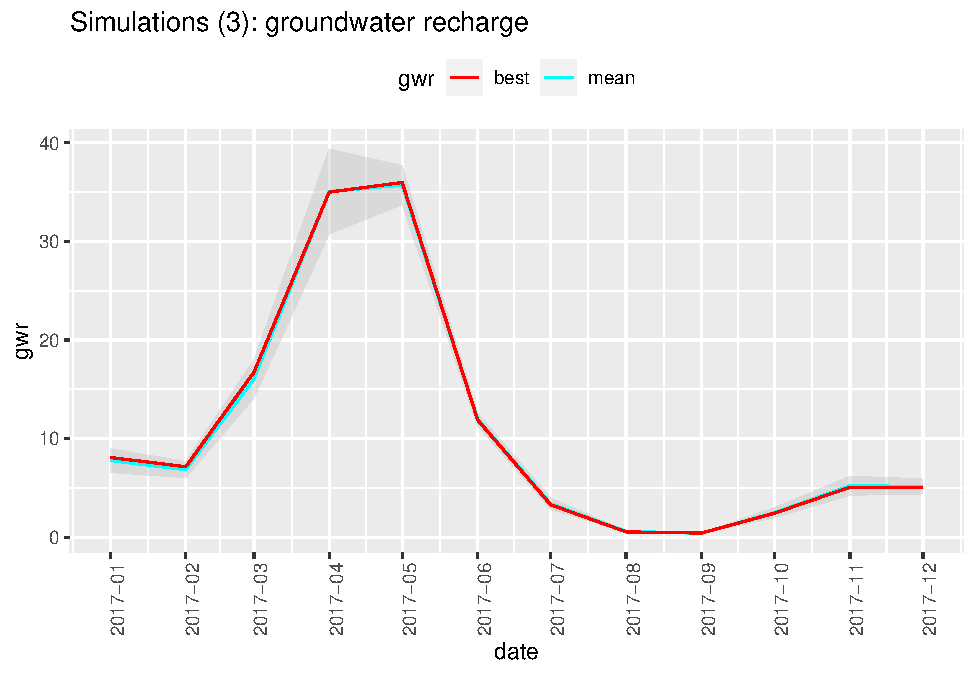
\includegraphics{fig/calib-uncert-gwr-1.pdf}

\begin{Shaded}
\begin{Highlighting}[]
\FunctionTok{plot\_metric}\NormalTok{(water\_budgets, }\StringTok{"runoff"}\NormalTok{, }
            \AttributeTok{title =} \FunctionTok{paste0}\NormalTok{(}\StringTok{"Simulations ("}\NormalTok{, }\FunctionTok{length}\NormalTok{(param\_ids),}\StringTok{"): runoff"}\NormalTok{))}
\end{Highlighting}
\end{Shaded}

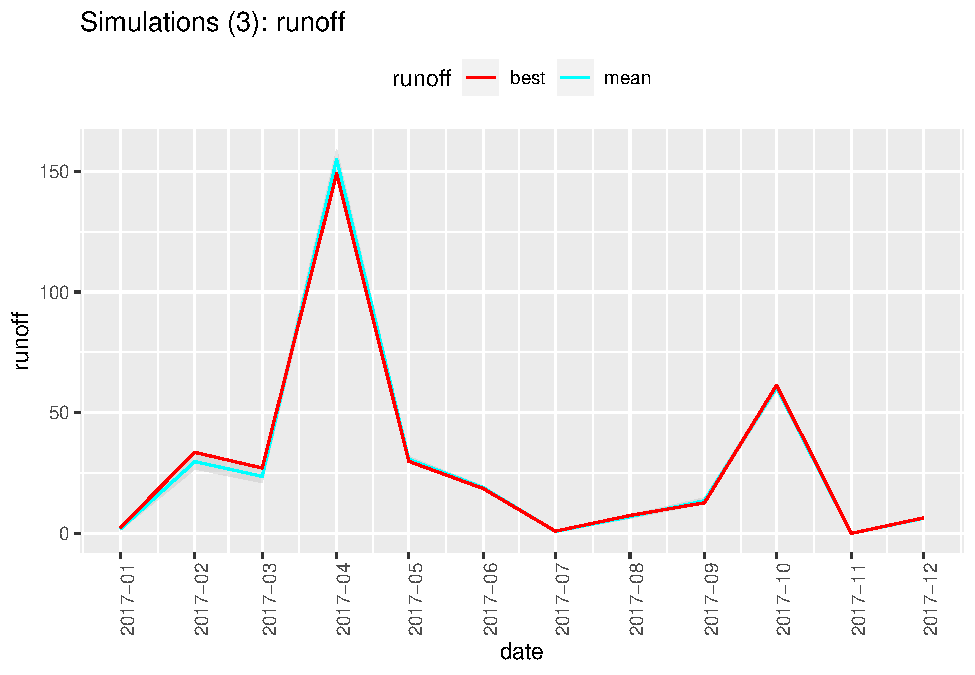
\includegraphics{fig/calib-uncert-runoff-1.pdf}

\begin{Shaded}
\begin{Highlighting}[]
\FunctionTok{plot\_metric}\NormalTok{(water\_budgets, }\StringTok{"vi"}\NormalTok{, }
            \AttributeTok{title =} \FunctionTok{paste0}\NormalTok{(}\StringTok{"Simulations ("}\NormalTok{, }\FunctionTok{length}\NormalTok{(param\_ids),}\StringTok{"): vertical inflow"}\NormalTok{))}
\end{Highlighting}
\end{Shaded}

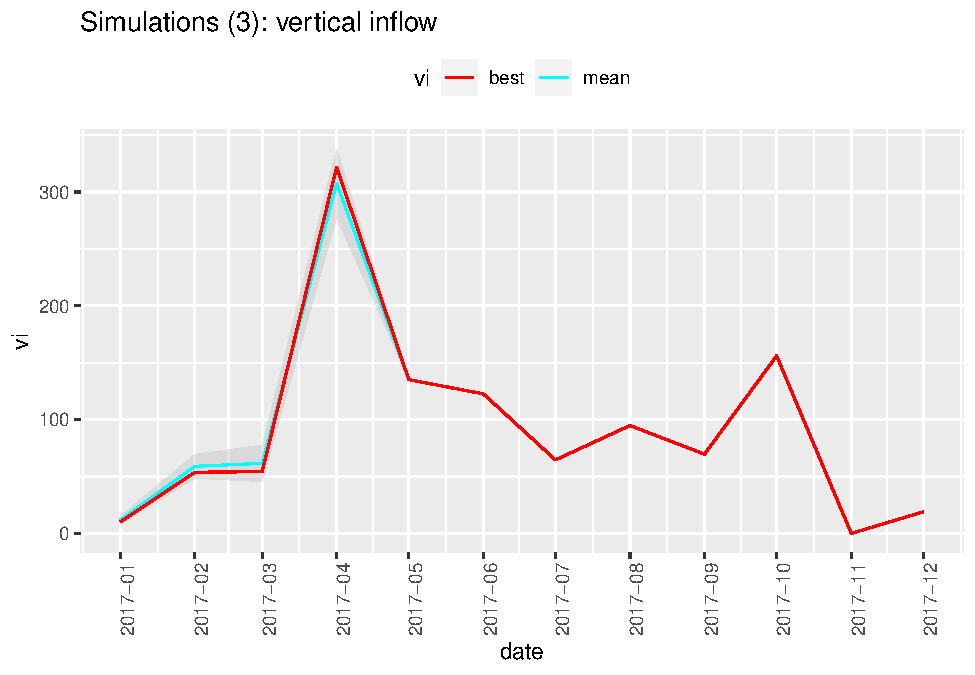
\includegraphics{fig/calib-uncert-vi-1.pdf}

\begin{Shaded}
\begin{Highlighting}[]
\FunctionTok{plot\_metric}\NormalTok{(water\_budgets, }\StringTok{"aet"}\NormalTok{, }
            \AttributeTok{title =} \FunctionTok{paste0}\NormalTok{(}\StringTok{"Simulations ("}\NormalTok{, }\FunctionTok{length}\NormalTok{(param\_ids),}\StringTok{"): actual evapotranspiration"}\NormalTok{))}
\end{Highlighting}
\end{Shaded}

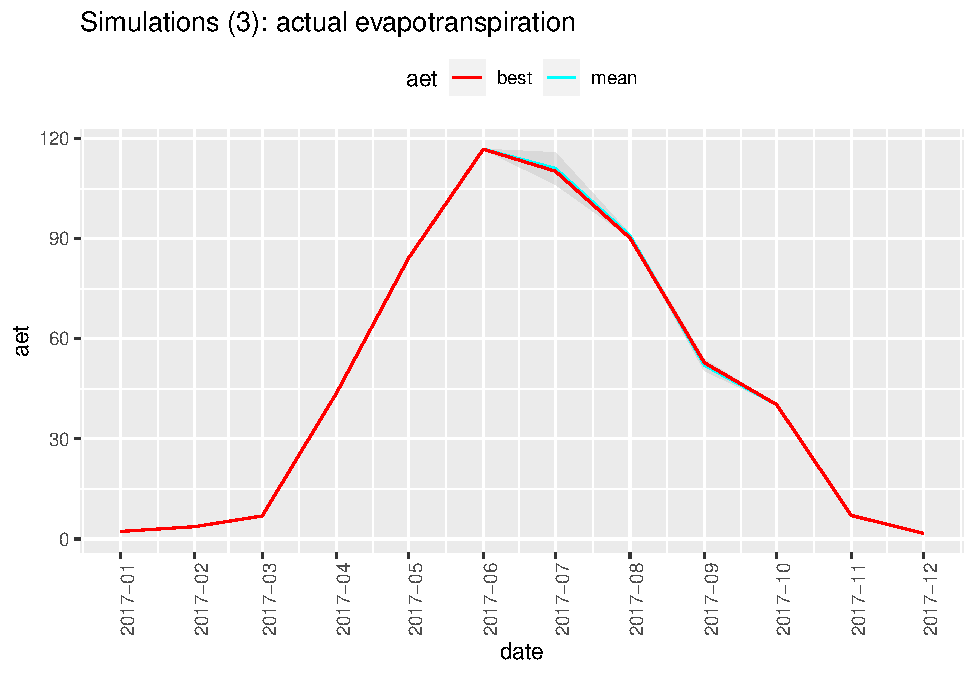
\includegraphics{fig/calib-uncert-aet-1.pdf}

\hypertarget{extensibility}{%
\chapter{Extensibility}\label{extensibility}}

\hypertarget{generic-functions}{%
\section{Generic functions}\label{generic-functions}}

The \texttt{rechaRge} package exposes the following \href{https://adv-r.hadley.nz/s3.html}{S3} generic functions:

\begin{itemize}
\tightlist
\item
  \href{https://gwrecharge.github.io/rechaRge/reference/compute_recharge.html}{\texttt{compute\_recharge}}, is the main function that performs the simulation computations according to the provided model parameters and input data. The result of this function is an input of the following functions.
\item
  \href{https://gwrecharge.github.io/rechaRge/reference/write_recharge_results.html}{\texttt{write\_recharge\_results}}, will write the simulation results into data files, summarized results can be included and various output file formats can be supported, depending on the model.
\item
  \href{https://gwrecharge.github.io/rechaRge/reference/write_recharge_rasters.html}{\texttt{write\_recharge\_rasters}}, will write the simulation results into raster files.
\item
  \href{https://gwrecharge.github.io/rechaRge/reference/evaluate_simulation_quality.html}{\texttt{evaluate\_simulation\_quality}}, is evaluating the quality of simulation output. This function should be used when making calibration and sensitivity analysis.
\end{itemize}

You can use the reference implementation of \textbf{HydroBudget} model to extend this API with your own model. For this you will need to start with the definition of a model specific object. In the case of \textbf{HydroBudget}, this object holds the parameters of the model and some helper information about the input source format. See the \href{https://gwrecharge.github.io/rechaRge/reference/new_hydrobudget.html}{\texttt{new\_hydrobudget}} function.

\hypertarget{other-languages}{%
\section{Other languages}\label{other-languages}}

If you have a model designed in Python, you could consider using the \href{https://rstudio.github.io/reticulate/}{\texttt{reticulate}} R package that facilitates the binding between the R and the Python execution environments.

\hypertarget{about-r}{%
\chapter{About R}\label{about-r}}

R is a free, open-source software and programming language developed in 1995 at the University of Auckland as an environment for statistical computing and graphics \href{https://www.stat.auckland.ac.nz/~ihaka/downloads/R-paper.pdf}{(Ikaha and Gentleman, 1996)}. Since then R has become one of the dominant software environments for data analysis and is used by a variety of scientific disciplines. CRAN Tasks provides an excellent overview of existing R packages for a given discipline (see for instance \href{https://cran.r-project.org/web/views/Environmetrics.html}{Envirometrics Task View}; \href{https://cran.r-project.org/web/views/Spatial.html}{Spatial Task View}).

R offers numerous advantages, such as:

\begin{enumerate}
\def\labelenumi{\arabic{enumi}.}
\item
  \href{https://www.gnu.org/philosophy/free-sw.html}{Free and Open source}
\item
  \href{http://christophergandrud.github.io/RepResR-RStudio/}{Reproducible Research}

  \begin{itemize}
  \tightlist
  \item
    repeatable:

    \begin{itemize}
    \tightlist
    \item
      code + output in a single document
    \item
      easier the re-analyses
    \end{itemize}
  \item
    scalable: applicable to small or large datasets
  \item
    extensible: several
  \end{itemize}
\item
  Getting help

  \begin{itemize}
  \tightlist
  \item
    \href{https://cran.r-project.org/web/views/}{Numerous Discipline Specific R Groups}
  \item
    \href{https://jumpingrivers.github.io/meetingsR/r-user-groups.html\#north-america}{Numerous Local R User Groups (including R-Ladies Groups)}
  \item
    \href{https://stackoverflow.com/}{Stack Overflow}
  \end{itemize}
\item
  Learning Resources

  \begin{itemize}
  \tightlist
  \item
    \href{https://www.r-project.org/doc/bib/R-books.html}{R books}
  \item
    \href{https://bookdown.org/}{(Free Online) R Books}
  \end{itemize}
\end{enumerate}

  \bibliography{book.bib}

\end{document}
